\chapter{Analysis of Conservation of Midgut Transcriptional Response to Bloodfeeding in Four Vector Mosquitoes}
\todo[inline]{replace CITEME tags in Analysis of Conservation of Midgut Transcriptional Response to Bloodfeeding in Four Vector Mosquitoes}

\todo[inline]{write all the figures}

\todo[inline]{MEGA: you need to write most of this chapter}

\section{Background}
\begin{enumerate}
 \item Biological importance of bloodmeal to mosquito
 \item Biological importance of bloodmeal to transmission cyc
\end{enumerate}



\begin{figure}[hp]
% 
\begin{subfigure}[t]{.5\linewidth}
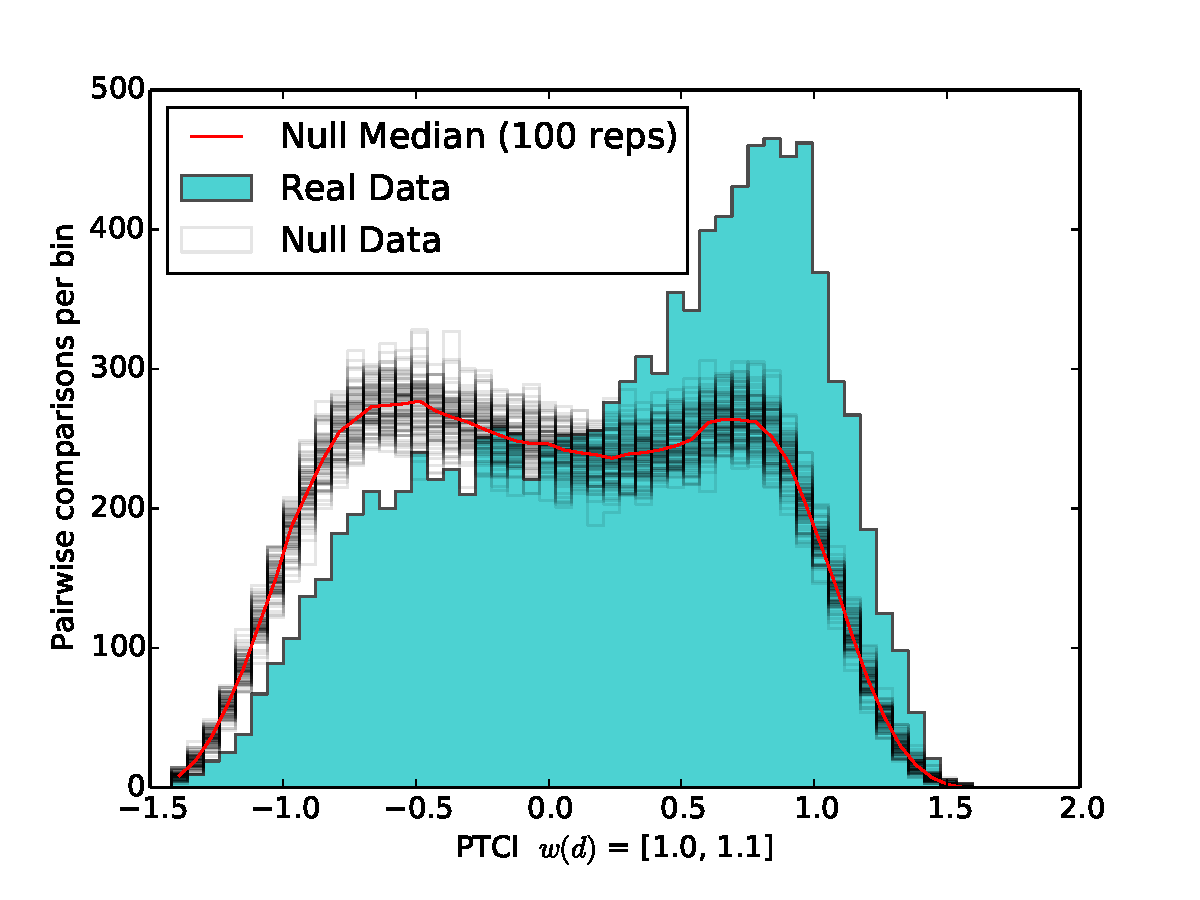
\includegraphics[width=\linewidth]{/home/gus/Dropbox/repos/git/uci-thesis-latex/figures/figs/ecr_team_ptci/pairwise_ptci_hist.pdf}
\caption{}
\label{fig:pairwise-ptci-hists-base}
\end{subfigure}%
\quad
\begin{subfigure}[t]{.5\linewidth}
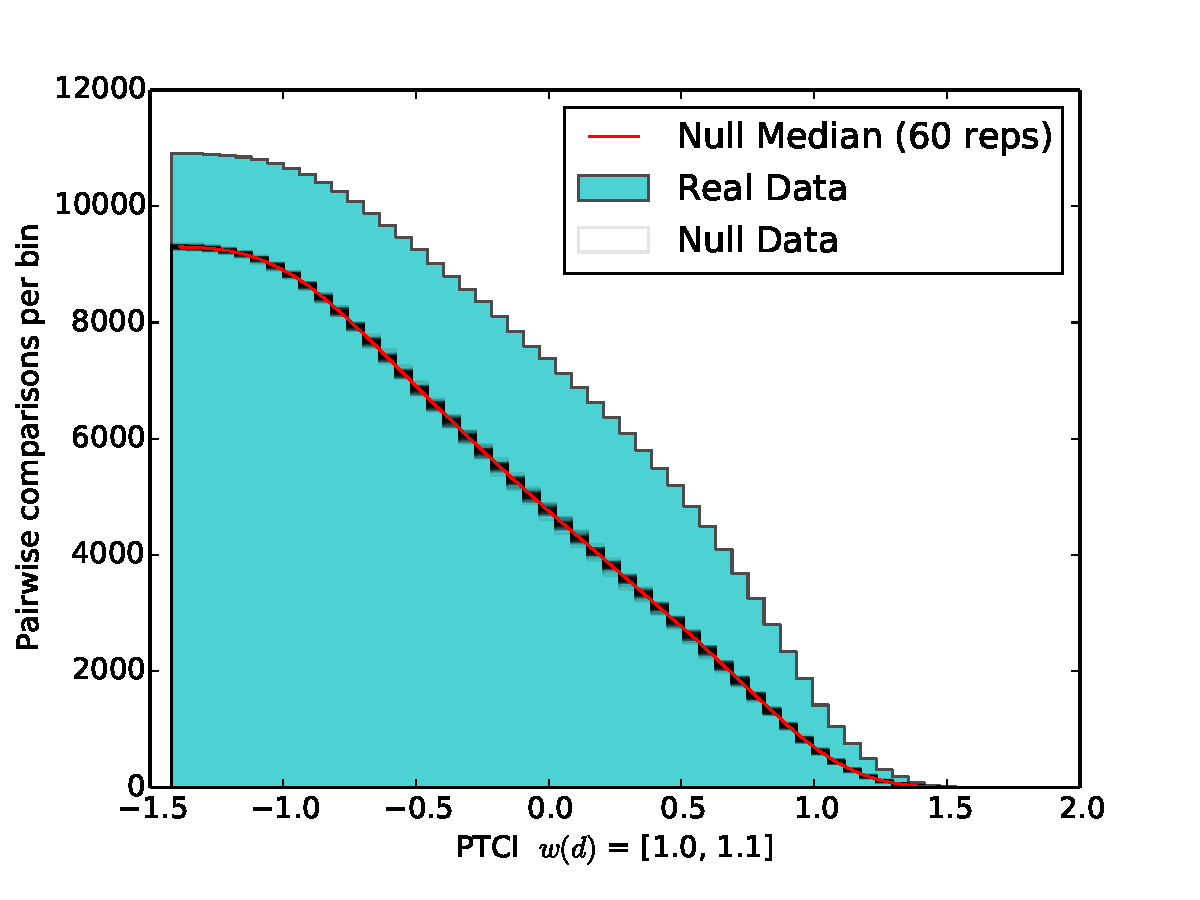
\includegraphics[width=\linewidth]{/home/gus/Dropbox/repos/git/uci-thesis-latex/figures/figs/ecr_team_ptci/pairwise_ptci_cum_hist.pdf}
\caption{}
\label{fig:pairwise-ptci-hists-rcum-hist}
\end{subfigure}
% 
\begin{subfigure}[t]{.5\linewidth}
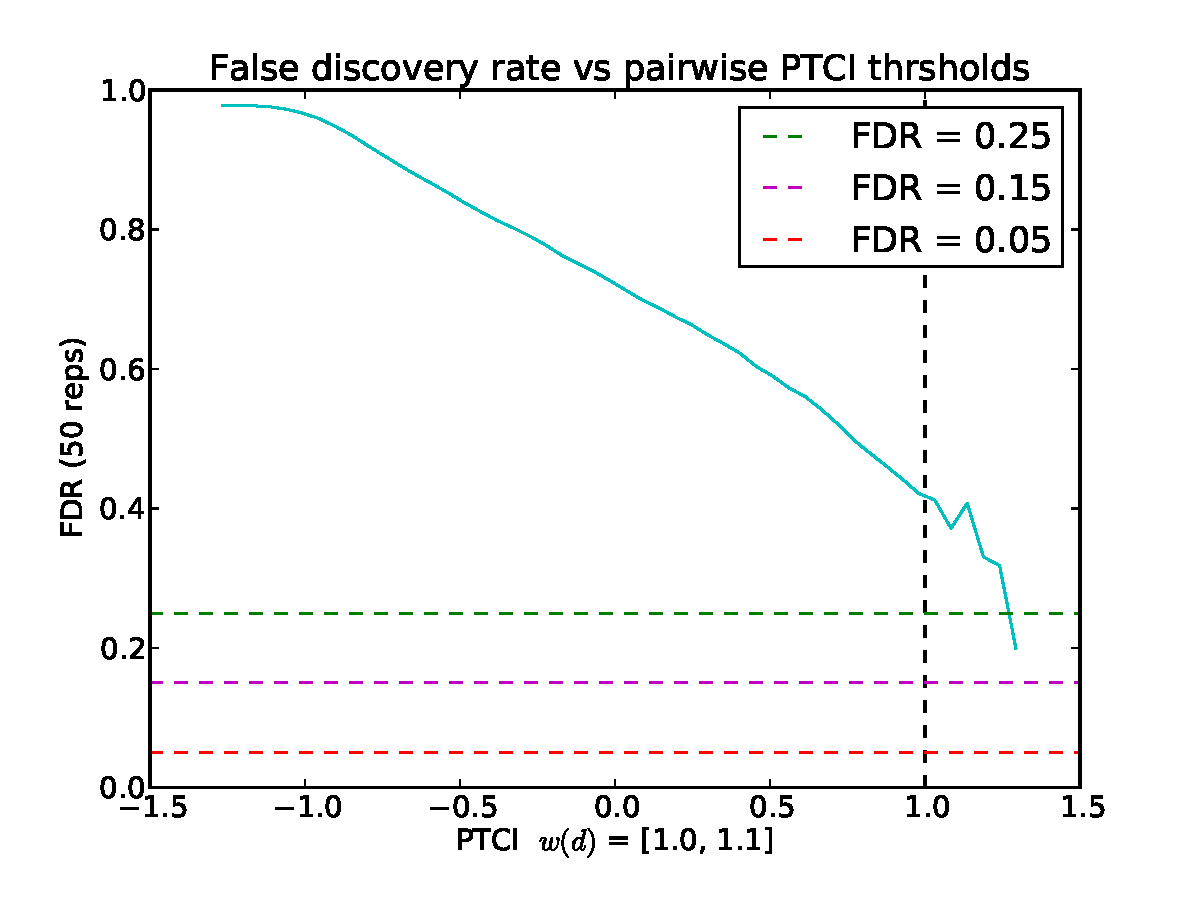
\includegraphics[width=\linewidth]{/home/gus/Dropbox/repos/git/uci-thesis-latex/figures/figs/ecr_team_ptci/pairwise_ptci_fdr.pdf}
\caption{}
\label{fig:pairwise-ptci-hists-fdr}
\end{subfigure}
% 
\caption[Pairwise PTCI results]{\sf \textbf{Pairwise PTCI results}:\\
\textbf{(A)} Histogram of pairwise PTCI results vs null distributions.
\textbf{(B)} Reverse Cumulative histogram of pairwise PTCI results vs null distributions.
\textbf{(C)} False discover rate vs PTCI threshold.}
\label{fig:pairwise-ptci-hists}
\end{figure}
Figure \ref{fig:pairwise-ptci-hists}


\begin{figure}[hp]
%
\subcaptionbox{\label{fig:mean-ptci-hists-base}}
{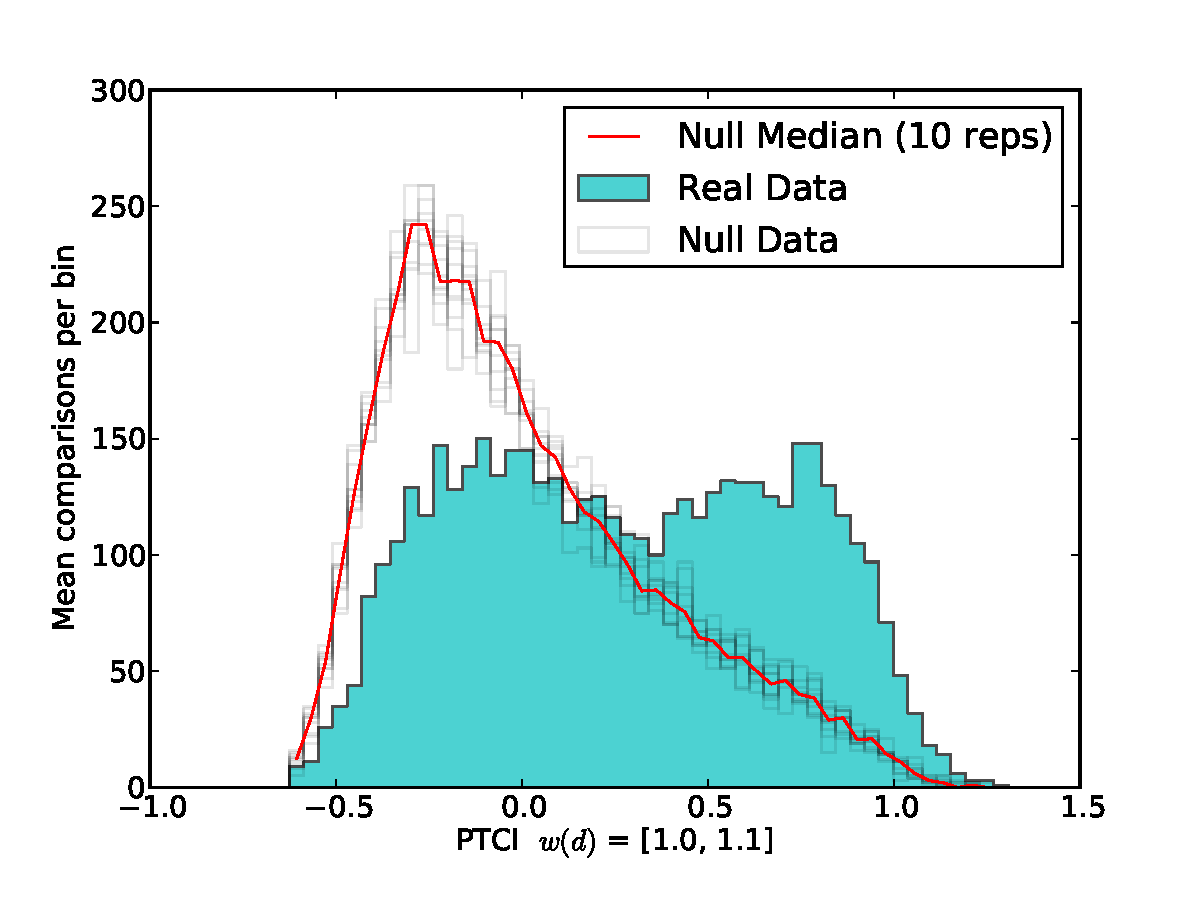
\includegraphics[width=.5\linewidth]{figures/figs/ecr_team_ptci/mean_ptci_hist.pdf}}
% 
\subcaptionbox{\label{fig:mean-ptci-hists-rcum-hist}}
{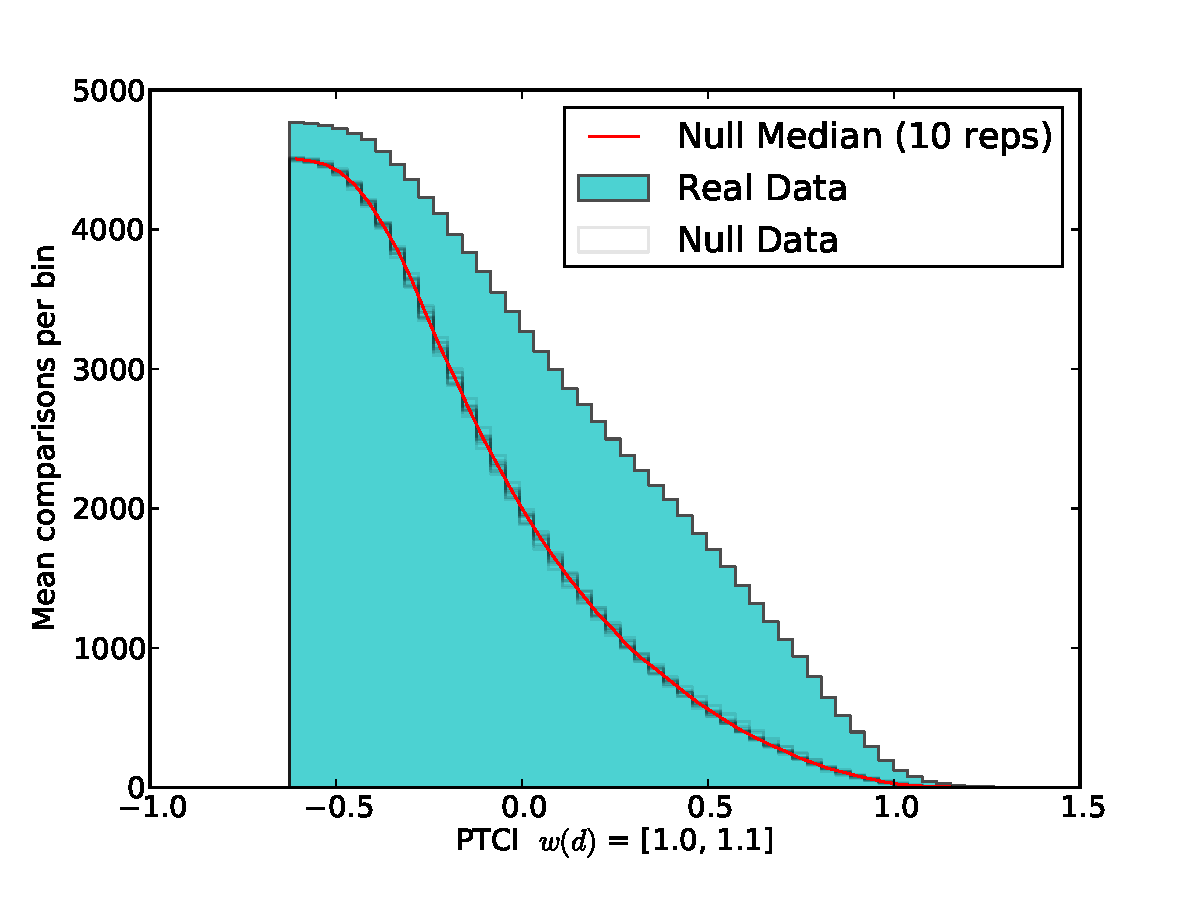
\includegraphics[width=.5\linewidth]{figures/figs/ecr_team_ptci/mean_ptci_cum_hist.pdf}}
% 
\subcaptionbox{\label{fig:mean-ptci-hists-fdr}}
{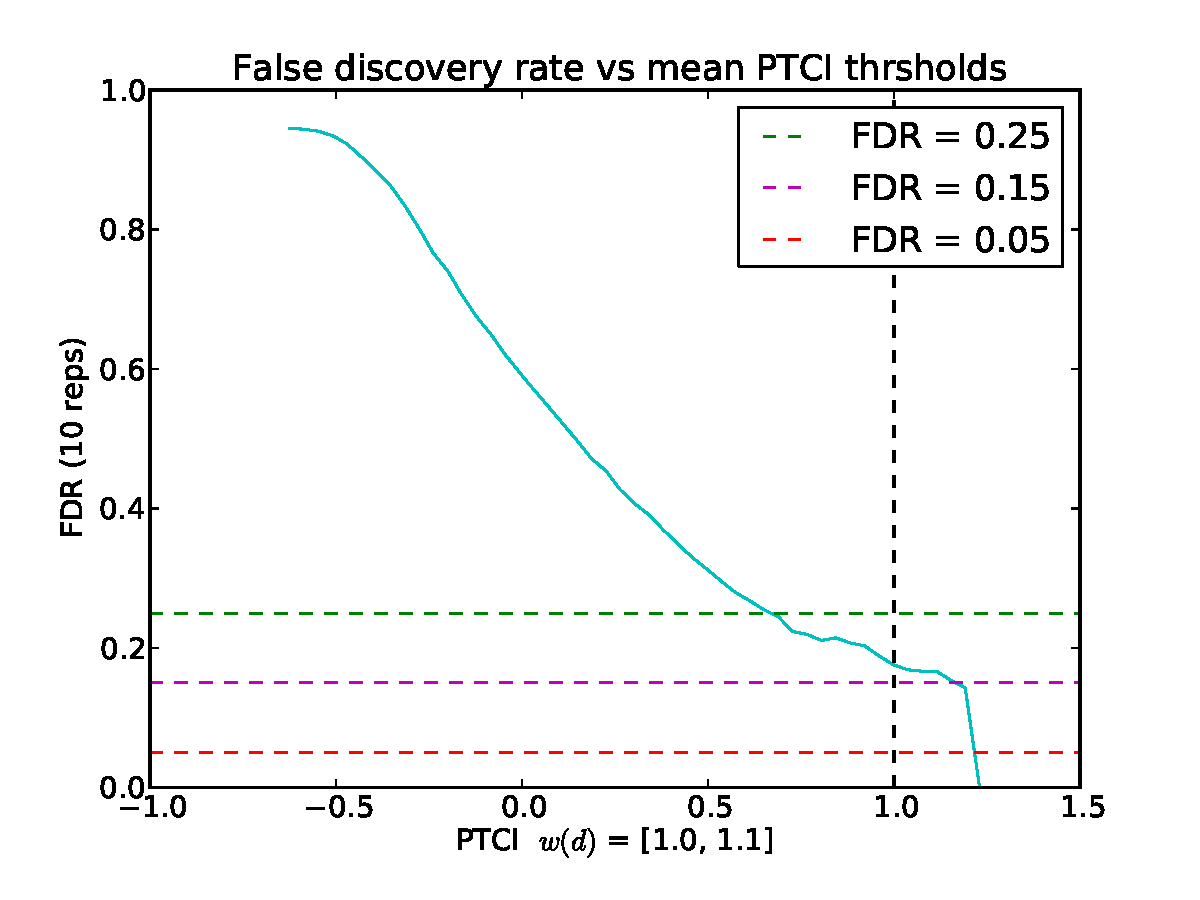
\includegraphics[width=.5\linewidth]{figures/figs/ecr_team_ptci/mean_ptci_fdr.pdf}}
% 
% 
\caption[Mean PTCI results]{\sf \textbf{Mean PTCI results}:\\
\textbf{(A)} Histogram of mean PTCI results vs null distributions.
\textbf{(B)} Reverse Cumulative histogram of mean PTCI results vs null distributions.
\textbf{(C)} False discover rate vs PTCI threshold.}
\label{fig:mean-ptci-hists}
\end{figure}
Figure \ref{fig:mean-ptci-hists}



\begin{landscape}

    \begin{figure}[h]
    \centering
    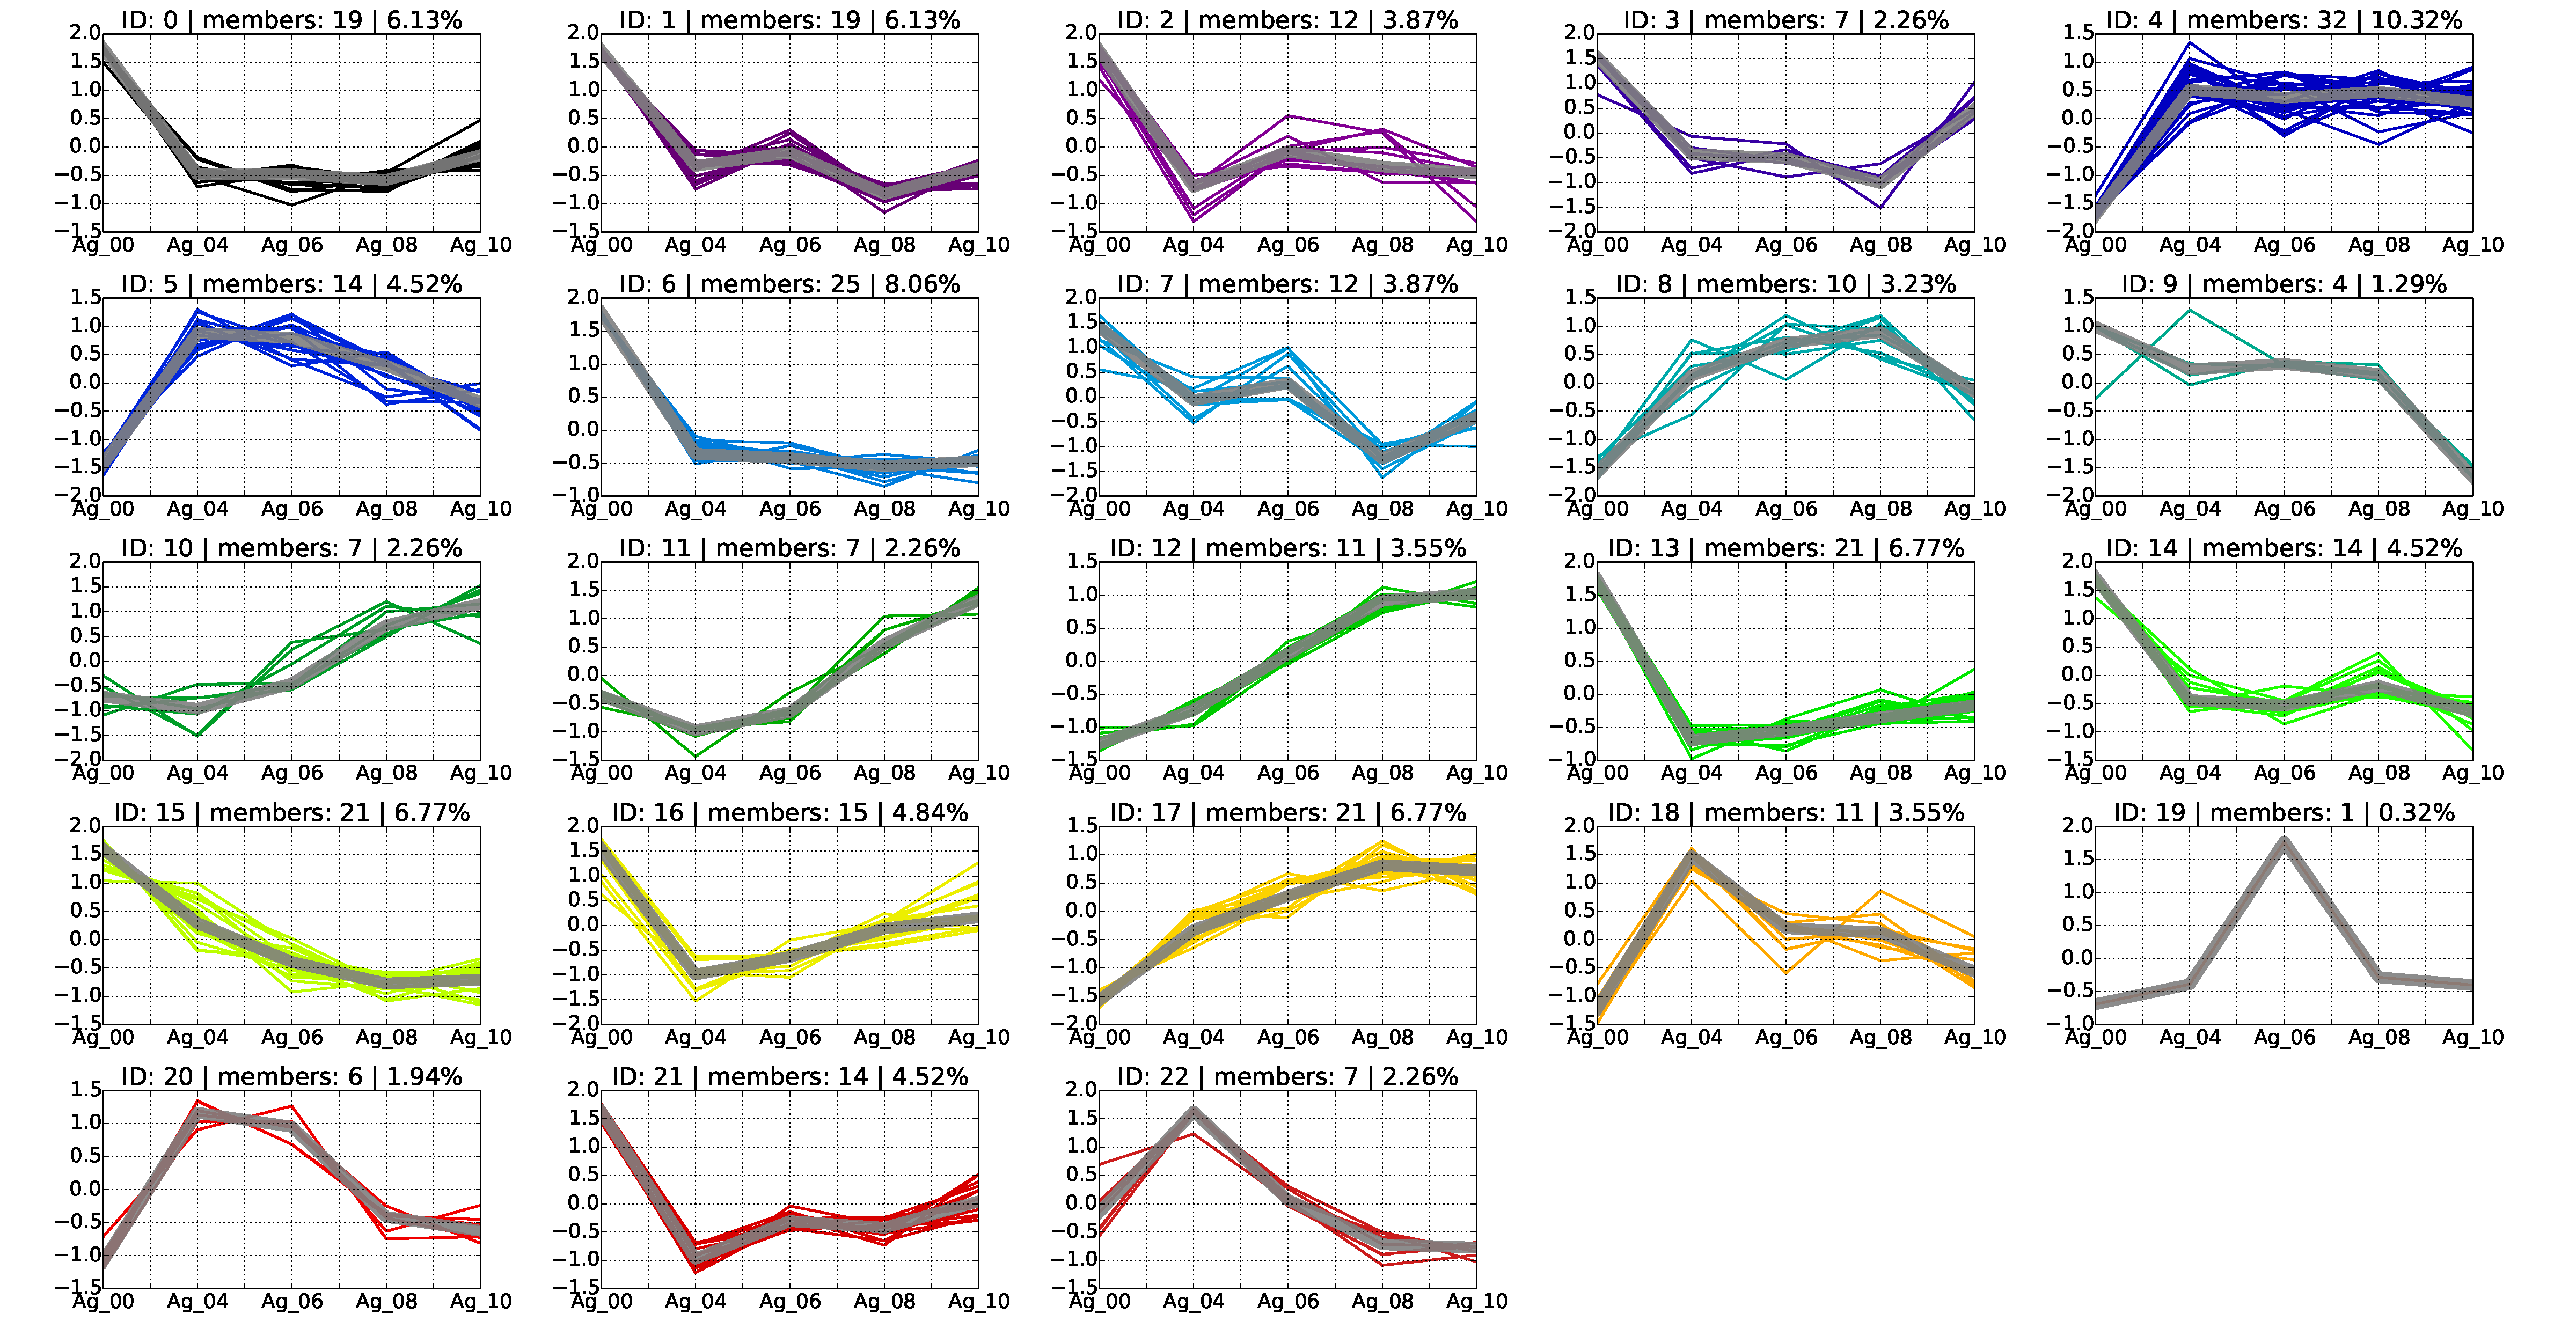
\includegraphics[width=\linewidth]{figures/figs/ecr_and_insects_ptci_20130918_orthodb7/23clusters_ptci_0_95_orthodb7.pdf}
    \caption[\Ag\ clustered abundance profiles]{\sf \textbf{\Ag\ clustered abundance profiles.} \\ 
    Clusters were generated using k-means clustering as implemented in Biopython version 1.62 \cite{Cock2009}.  Abundance profile data was log transformed after one FPKM was added to all data to remove zeros ($log_{10}(\mathrm{FPKM}+1)$).  K-means was then applied using the arithmetic mean as the center for cluster definition.  The data displayed here is the gene-wise standardization of the \textbf{raw} FPKM data such that each profile has mean = 0 and standard deviation = 1. Each median abundance profile is marked by a thick gray line. \textbf{Panel Titles} - ID: cluster identifier | members: number of genes in cluster | percentage of genes represented in all clusters. \textbf{Time Points} - \gls{NBF}, 4, 6, 8, 10 h \gls{PBM}.
}
    \label{fig:23-clusters}
    \end{figure}
    
\end{landscape}


Figure \ref{fig:23-clusters}

% 
\begin{figure}[hp]
% 
\subcaptionbox{\label{fig:cluster6-Aa}}
{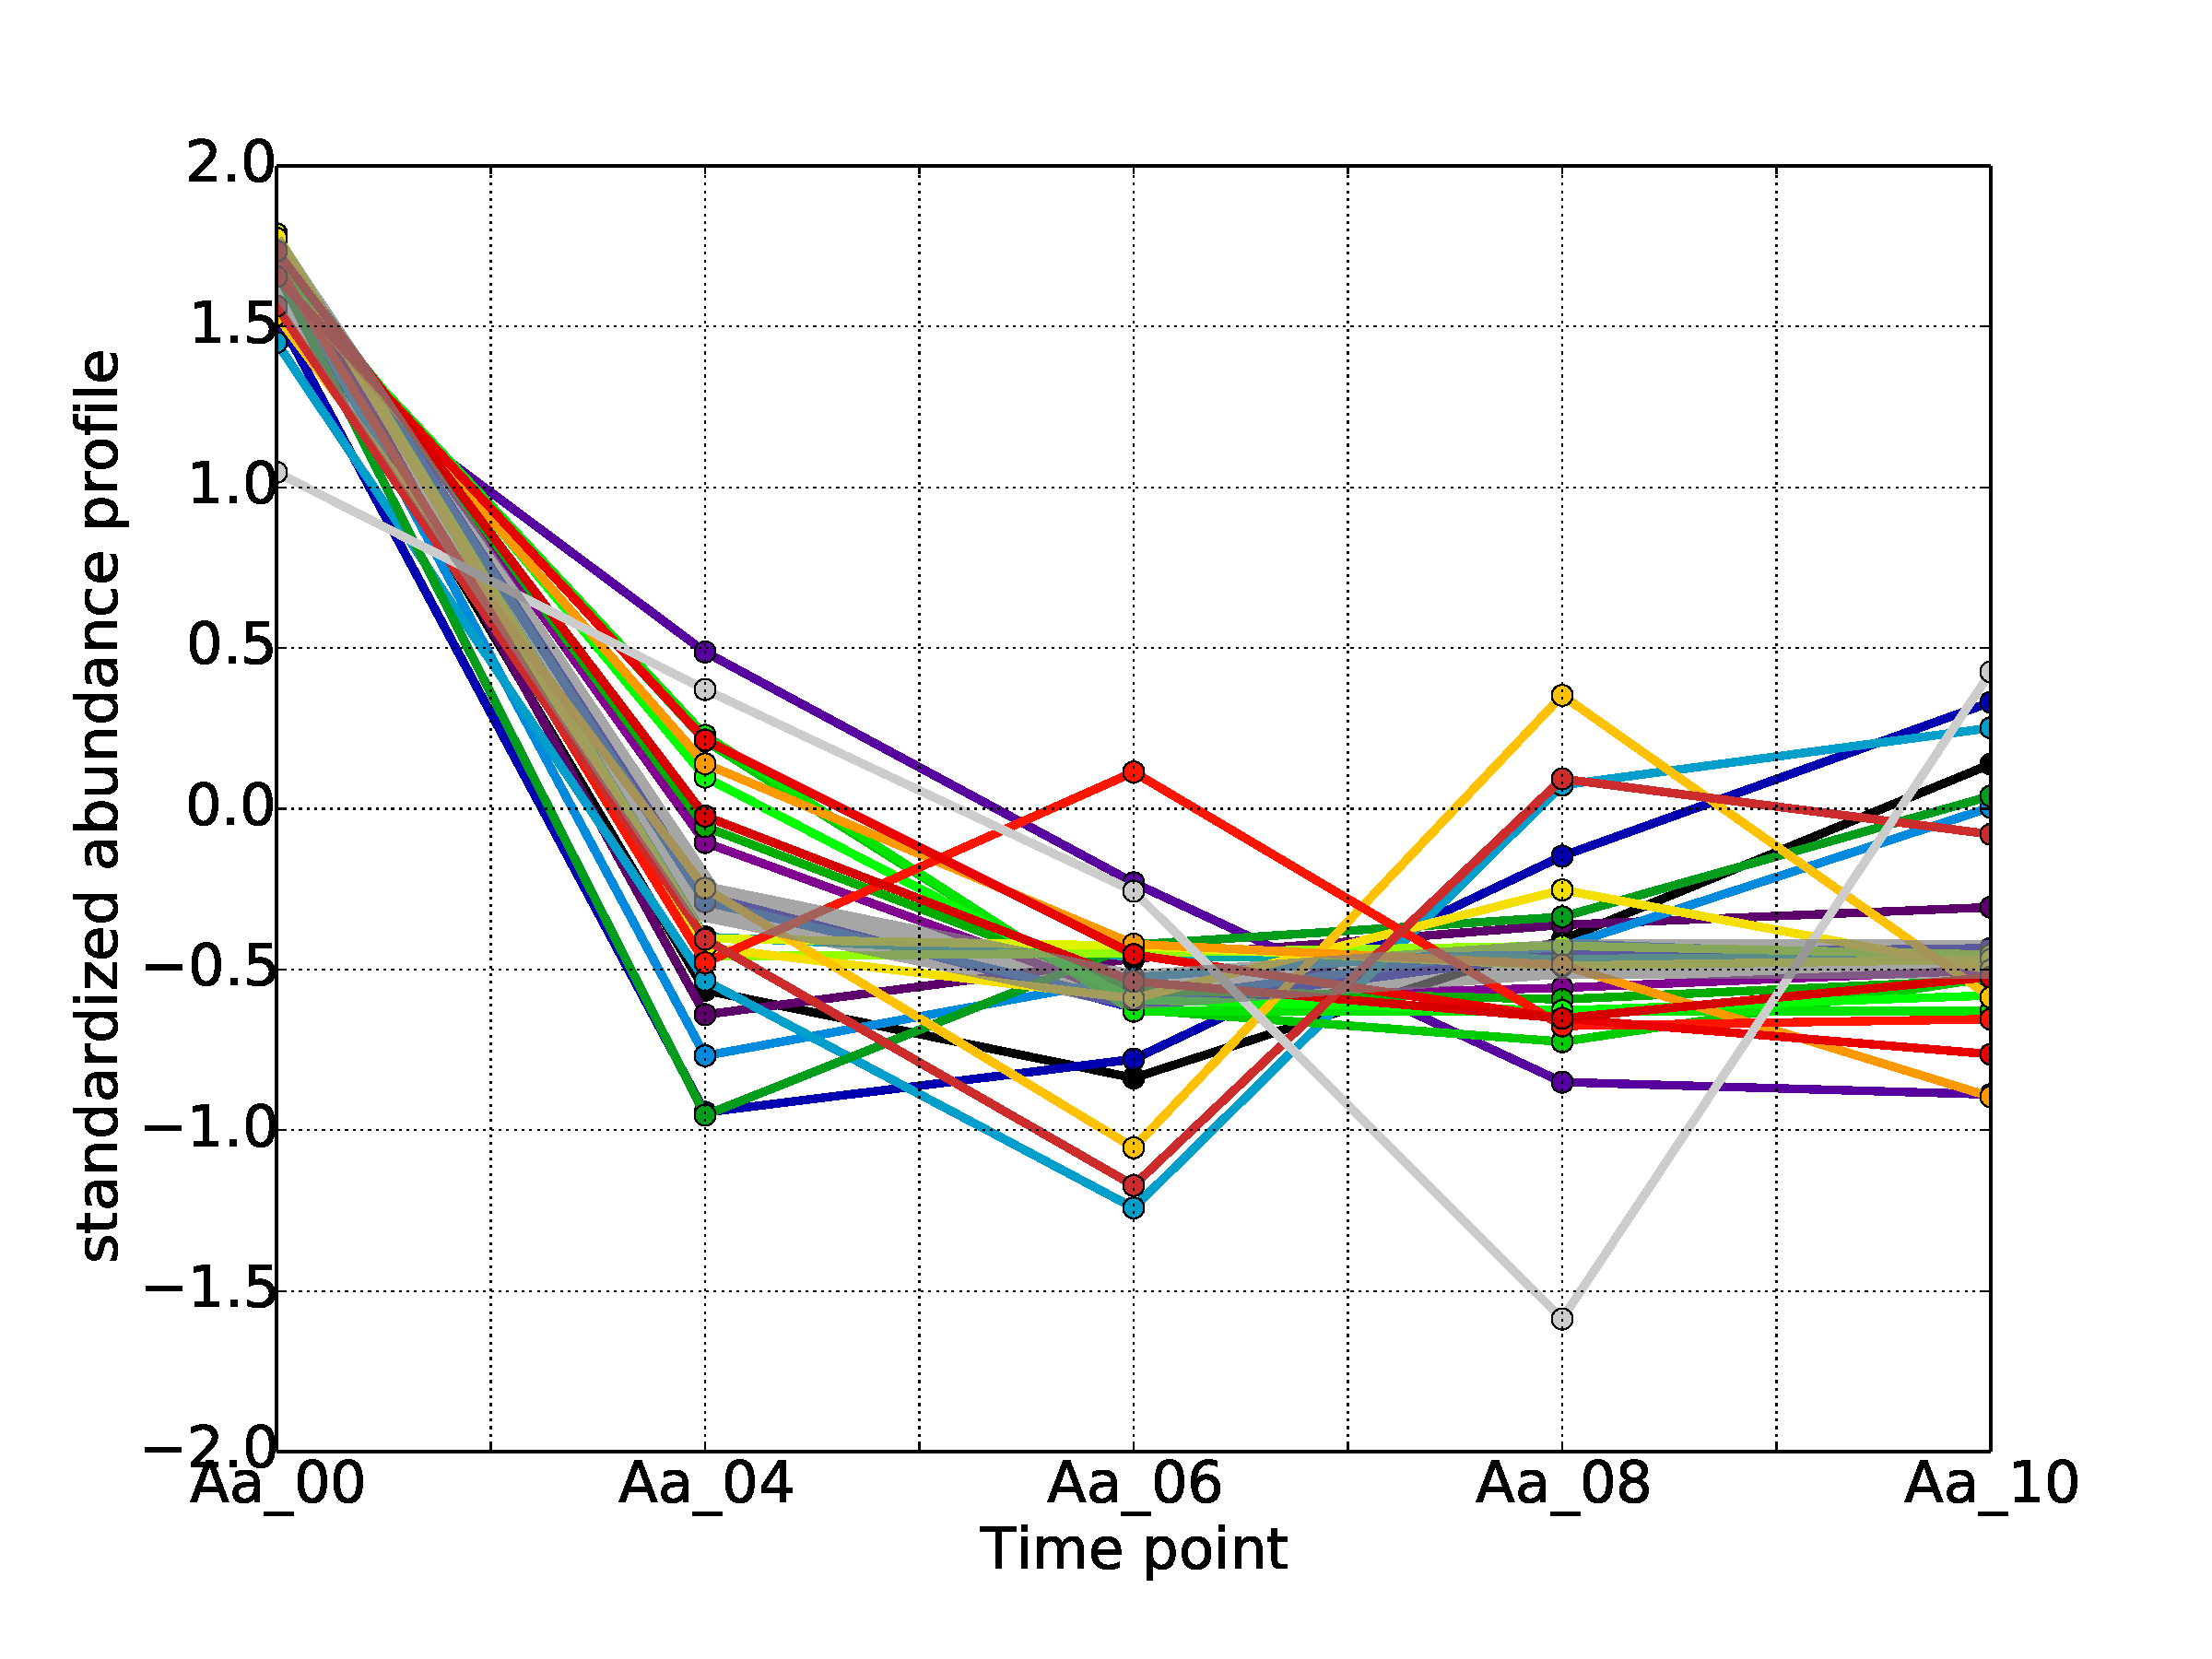
\includegraphics[width=.5\linewidth]{figures/figs/ecr_and_insects_ptci_20130918_orthodb7/downAfter4_gene_profiles_from_cummerbund/Aa_downAfter4_cls6_Ag_target_FPKMs_vb_orthos.pdf}}
%
\subcaptionbox{\label{fig:cluster6-Ag}}
{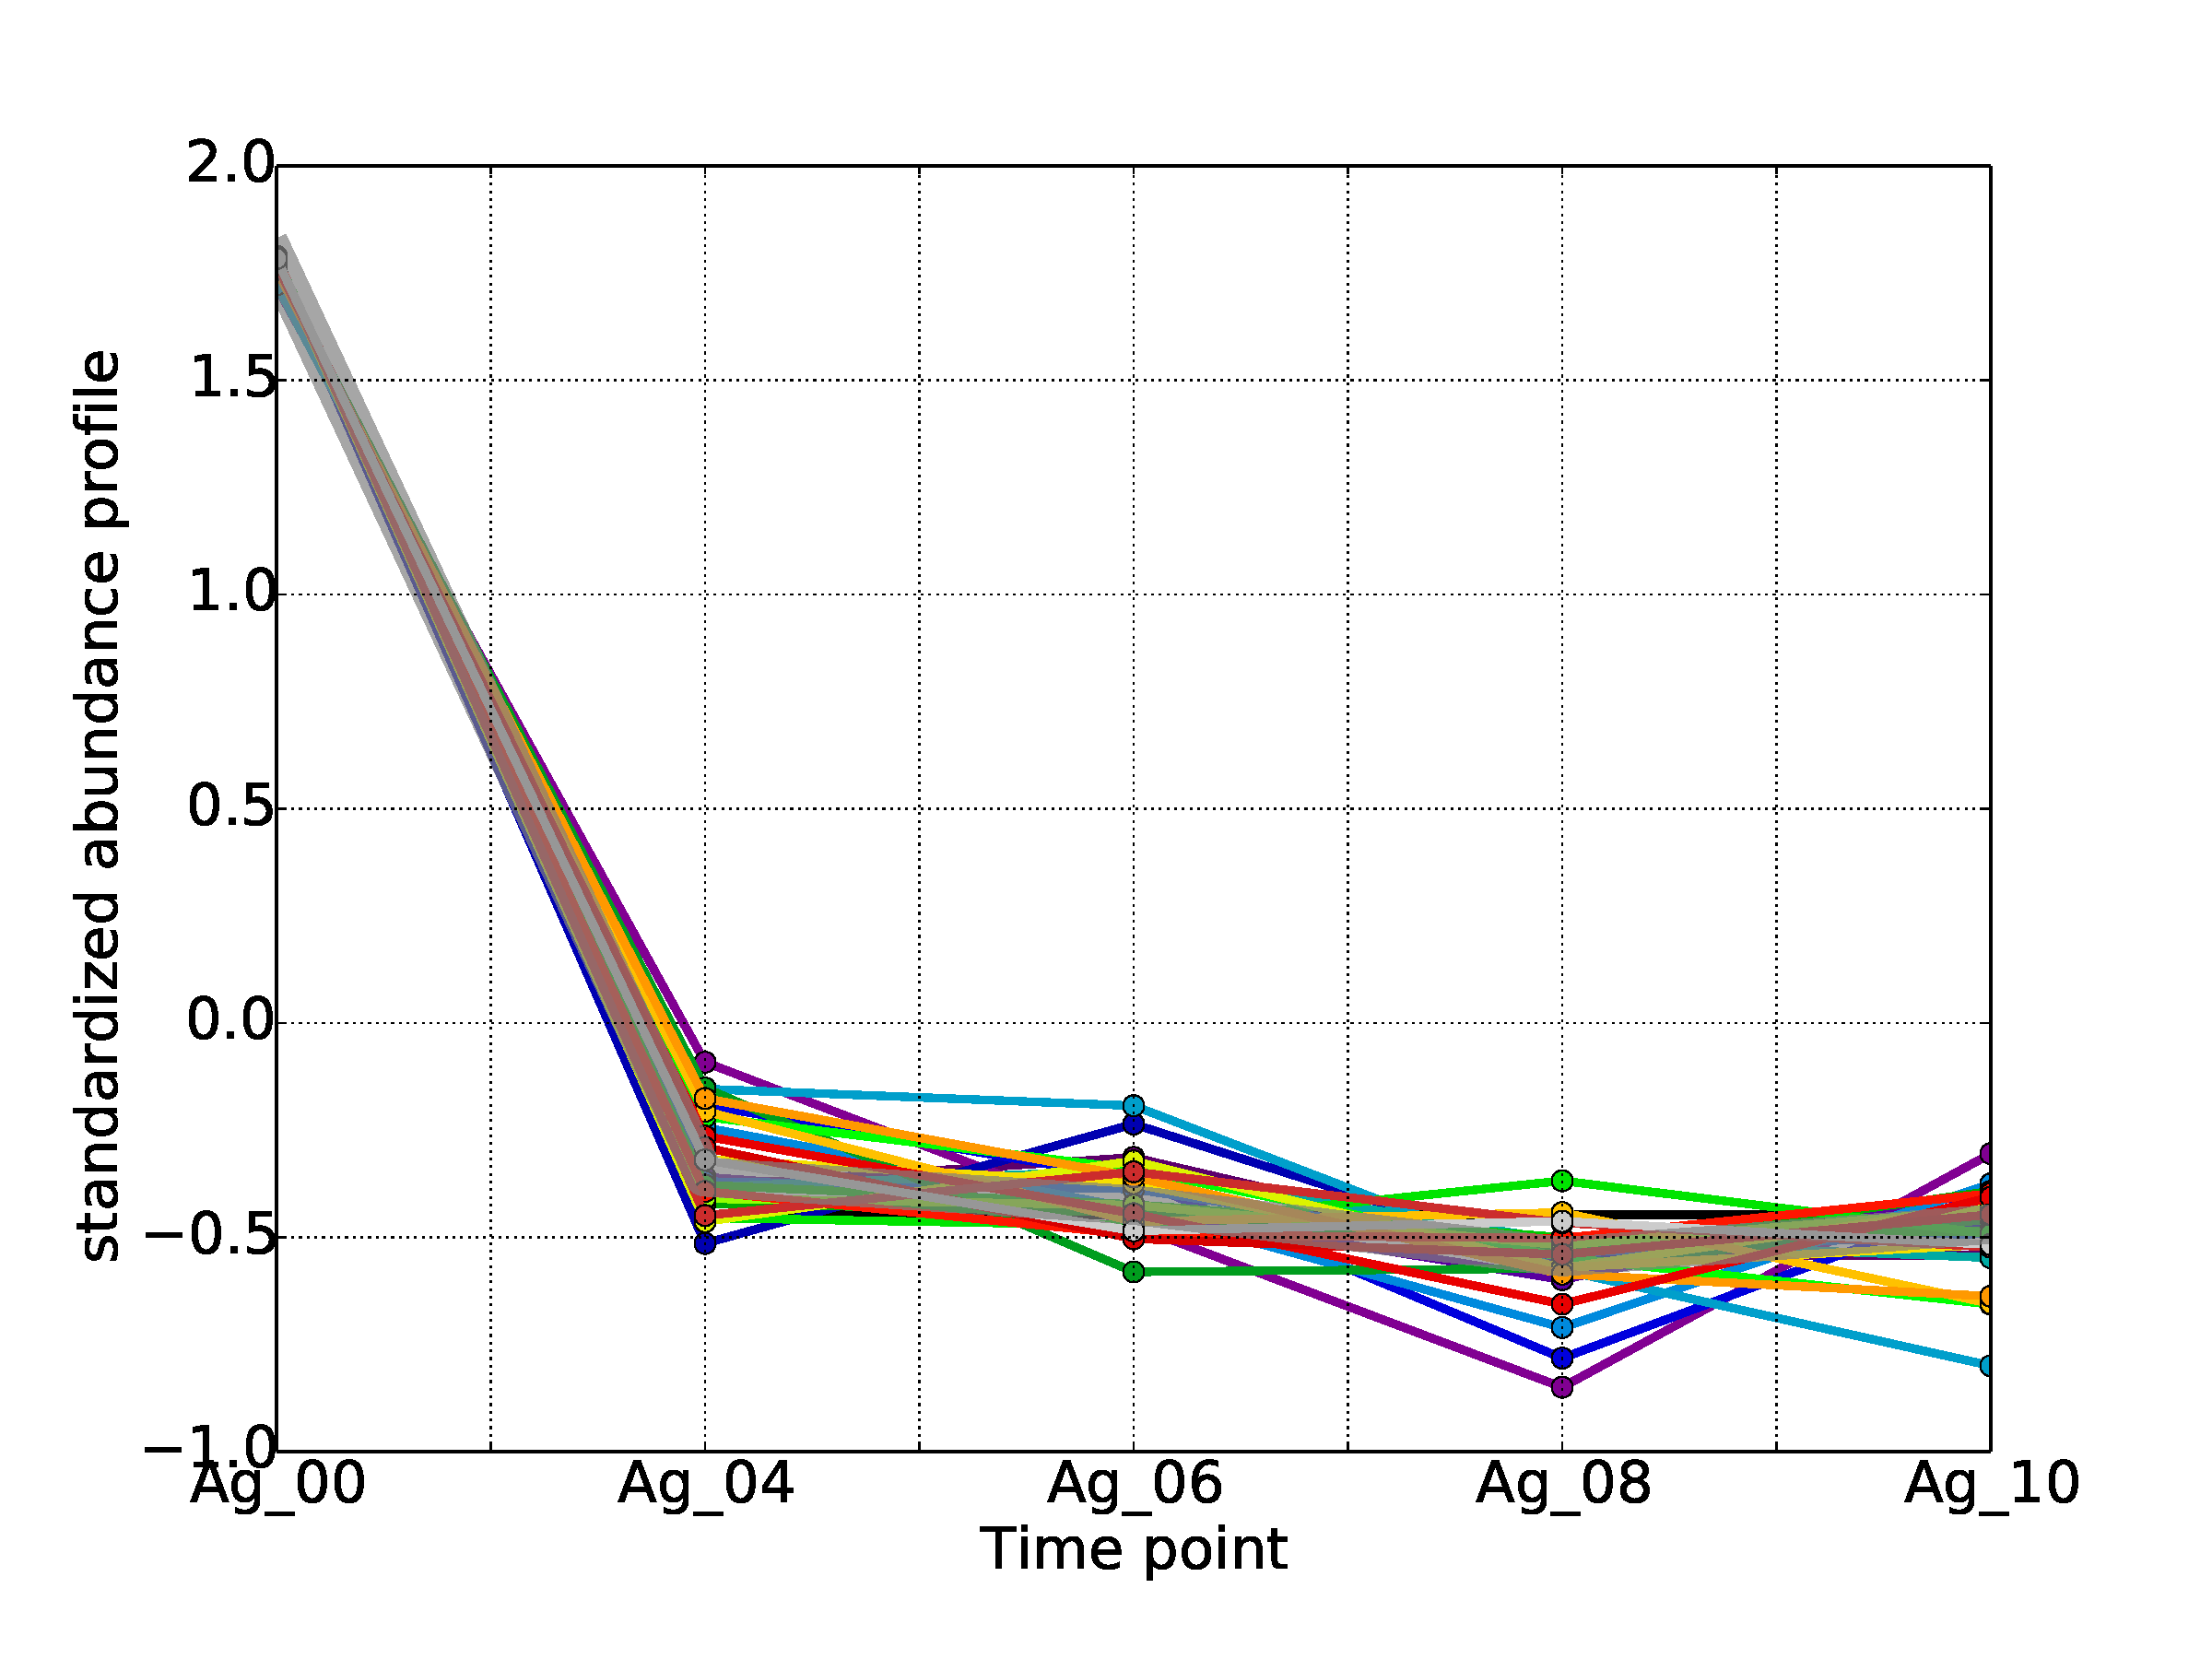
\includegraphics[width=.5\linewidth]{figures/figs/ecr_and_insects_ptci_20130918_orthodb7/downAfter4_gene_profiles_from_cummerbund/Ag_downAfter4_cls6_Ag_target_FPKMs_vb_orthos.pdf}}
%
\subcaptionbox{\label{fig:cluster6-Cq}}
{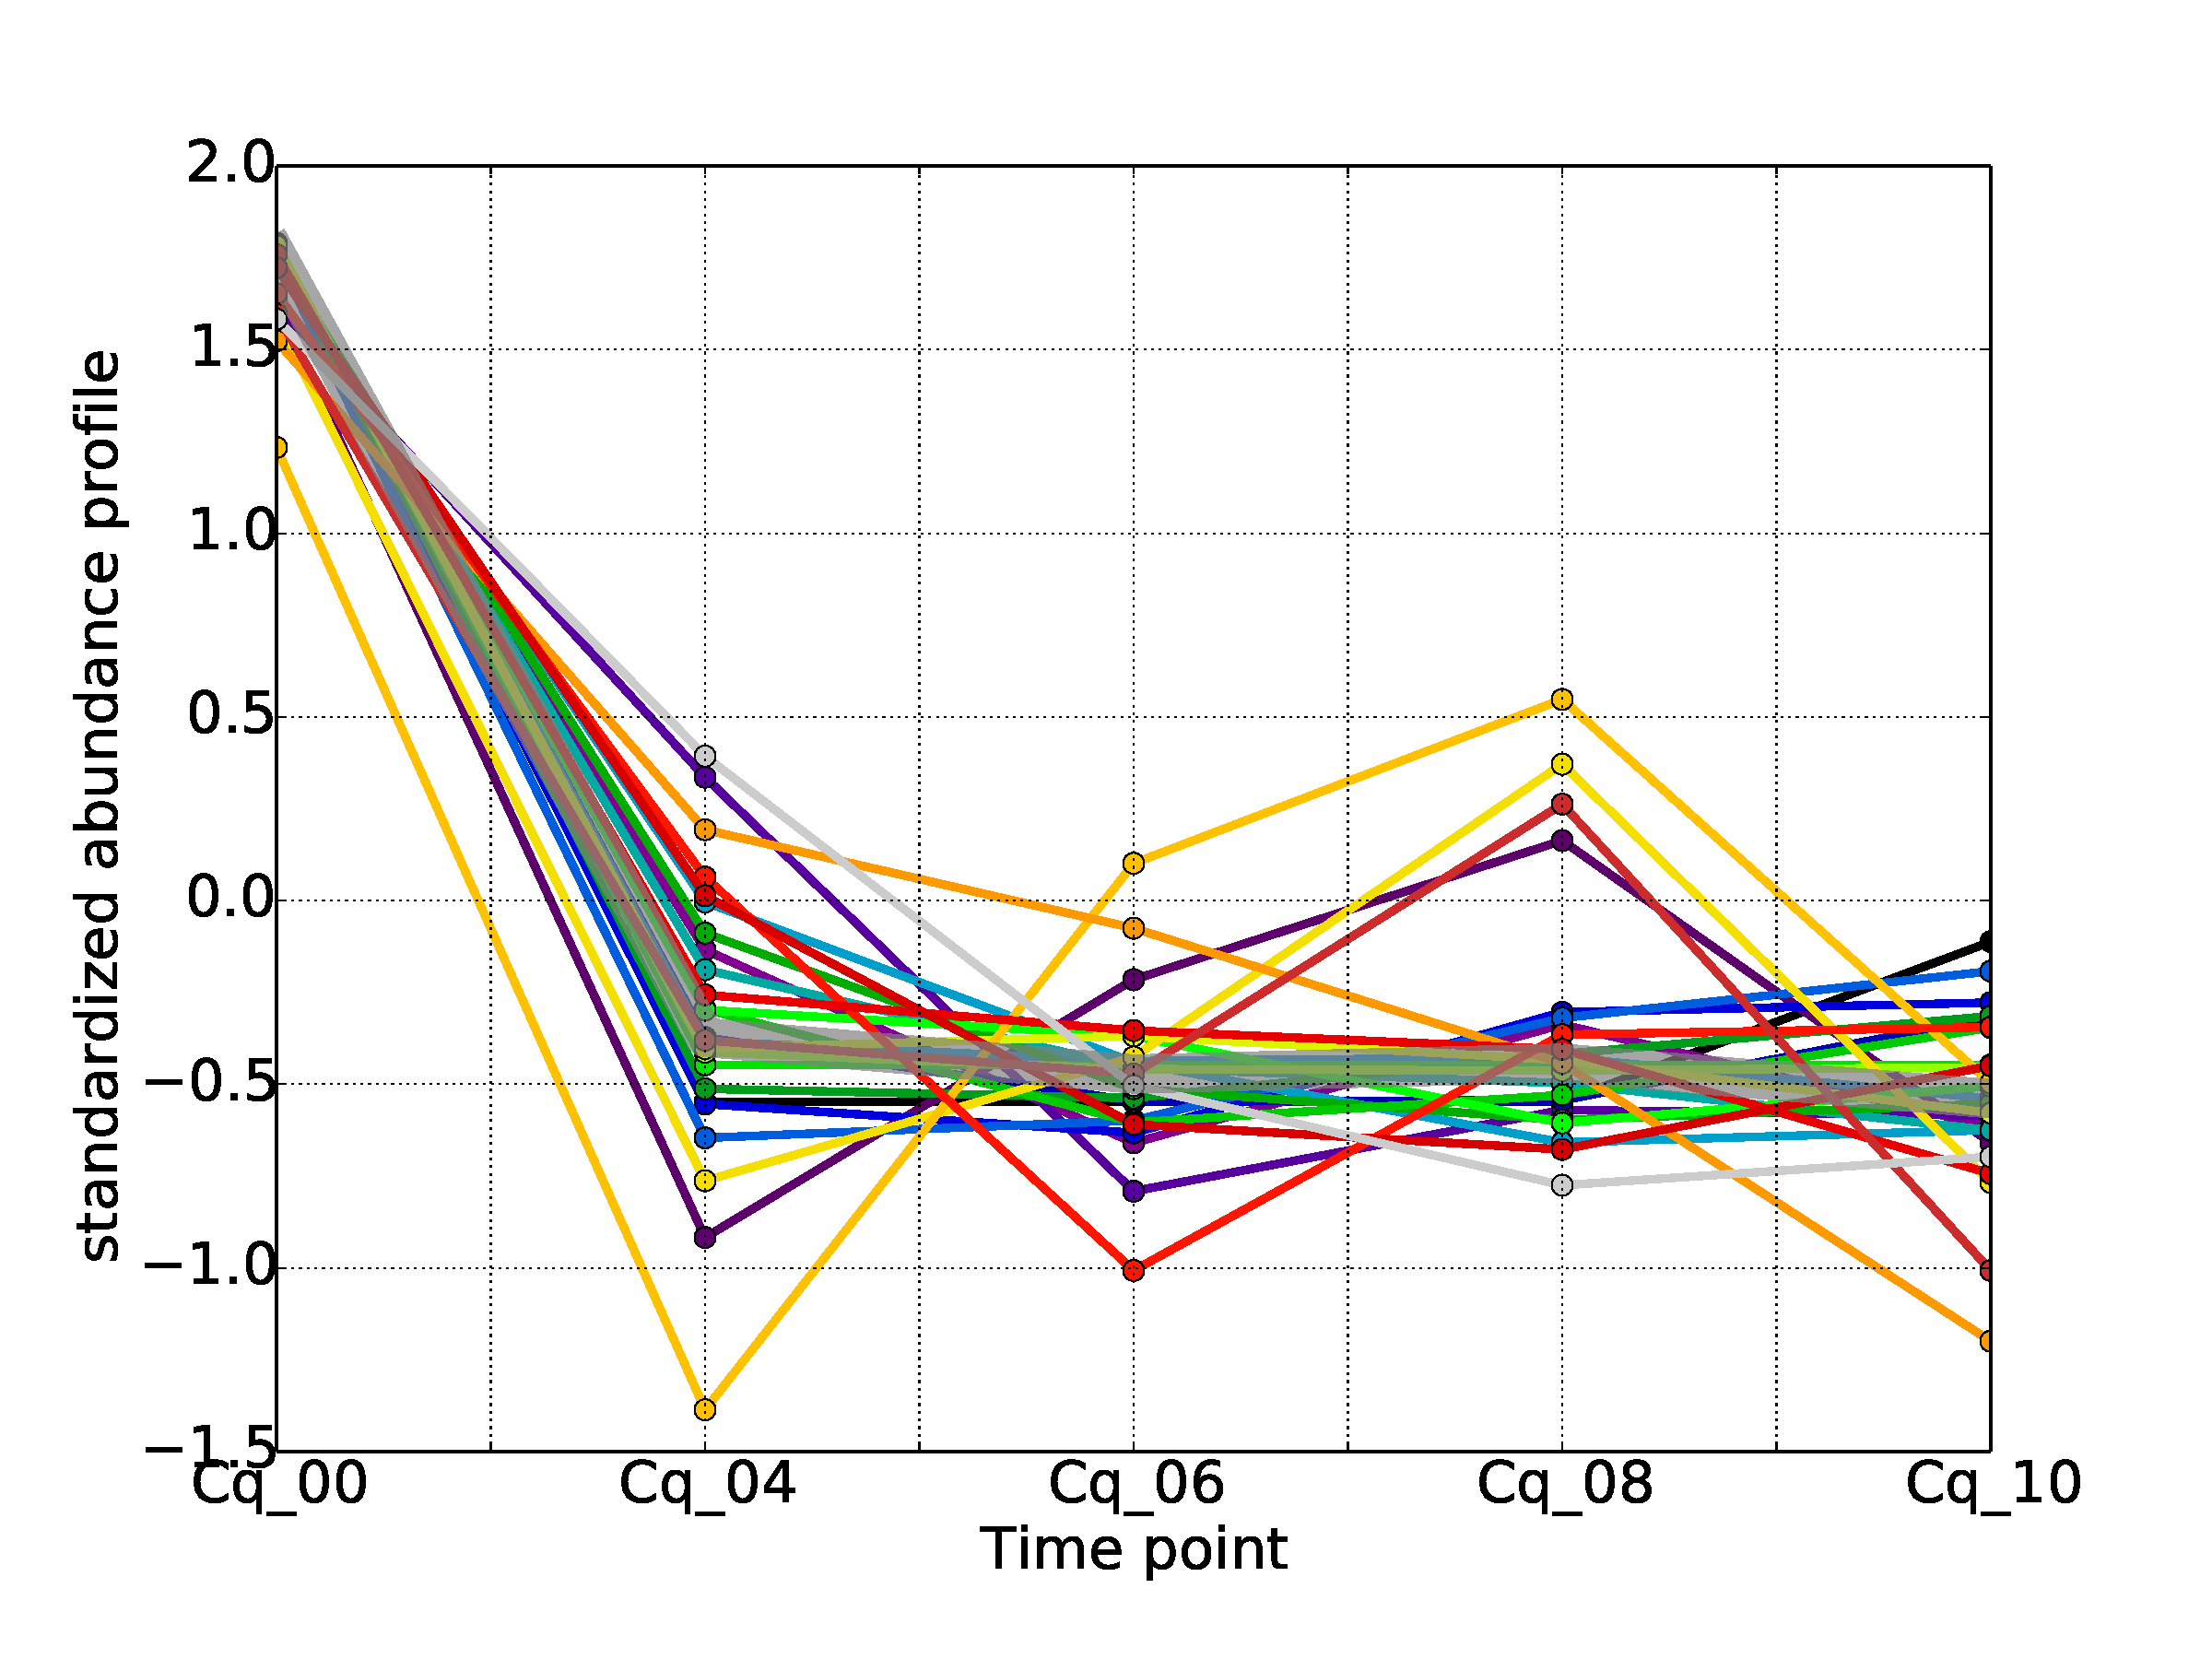
\includegraphics[width=.5\linewidth]{figures/figs/ecr_and_insects_ptci_20130918_orthodb7/downAfter4_gene_profiles_from_cummerbund/Cq_downAfter4_cls6_Ag_target_FPKMs_vb_orthos.pdf}}
% 
\caption[Orthologs of cluster 6]{\sf \textbf{Orthologs of cluster 6 (down after 4h):}\\
The same color scheme is used for each species which means that orthologs are given the same color in all three panels.
The thick, transparent gray line represents the median \gls{mAP} for the panel.
\textbf{(A)} \Aa.
\textbf{(B)} \Ag.
\textbf{(C)} \Cq.
}\label{fig:cluster6}
\end{figure}
% Figure \ref{fig:cluster6}
% 
% 
\begin{figure}[hp]
% 
\begin{subfigure}[t]{.5\linewidth}
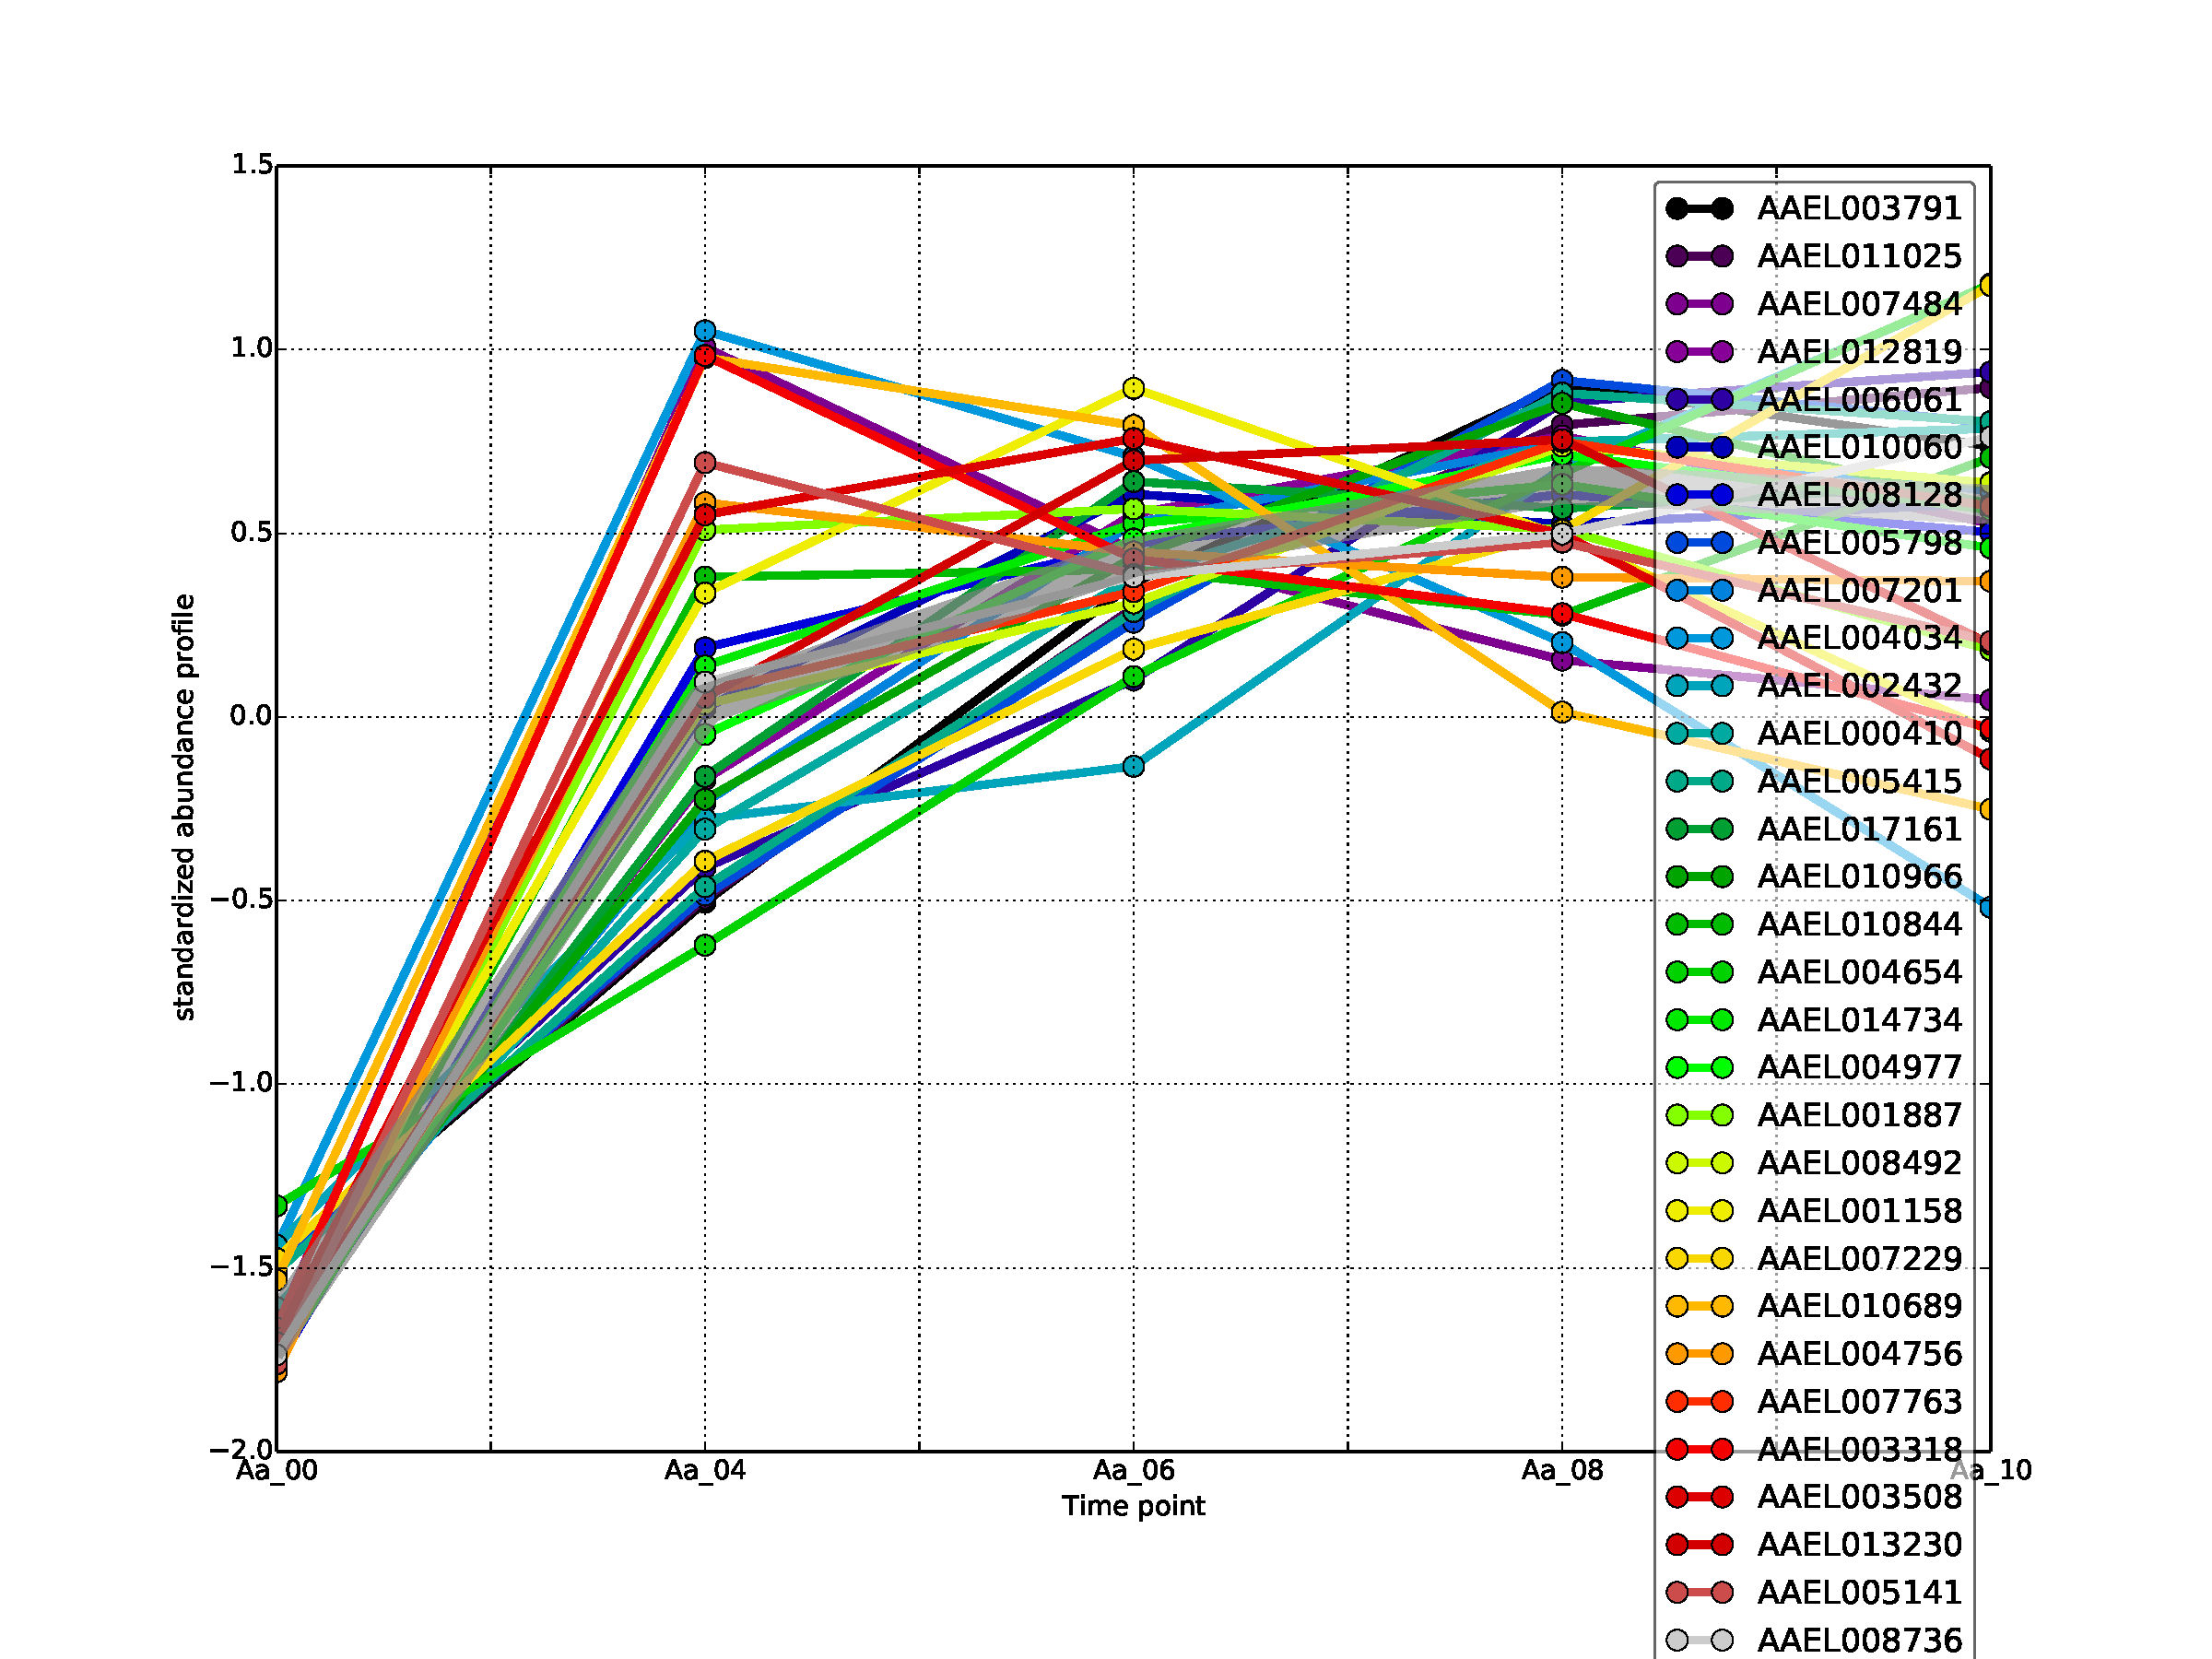
\includegraphics[width=\linewidth]{figures/figs/ecr_and_insects_ptci_20130903/upAfter4_gene_profiles_from_cummerbund/Aa_upAfter4_cls7_Ag_target_FPKMs_vb_orthos.pdf}
\caption{}
\label{fig:cluster7-Aa}
\end{subfigure}%
%
\begin{subfigure}[t]{.5\linewidth}
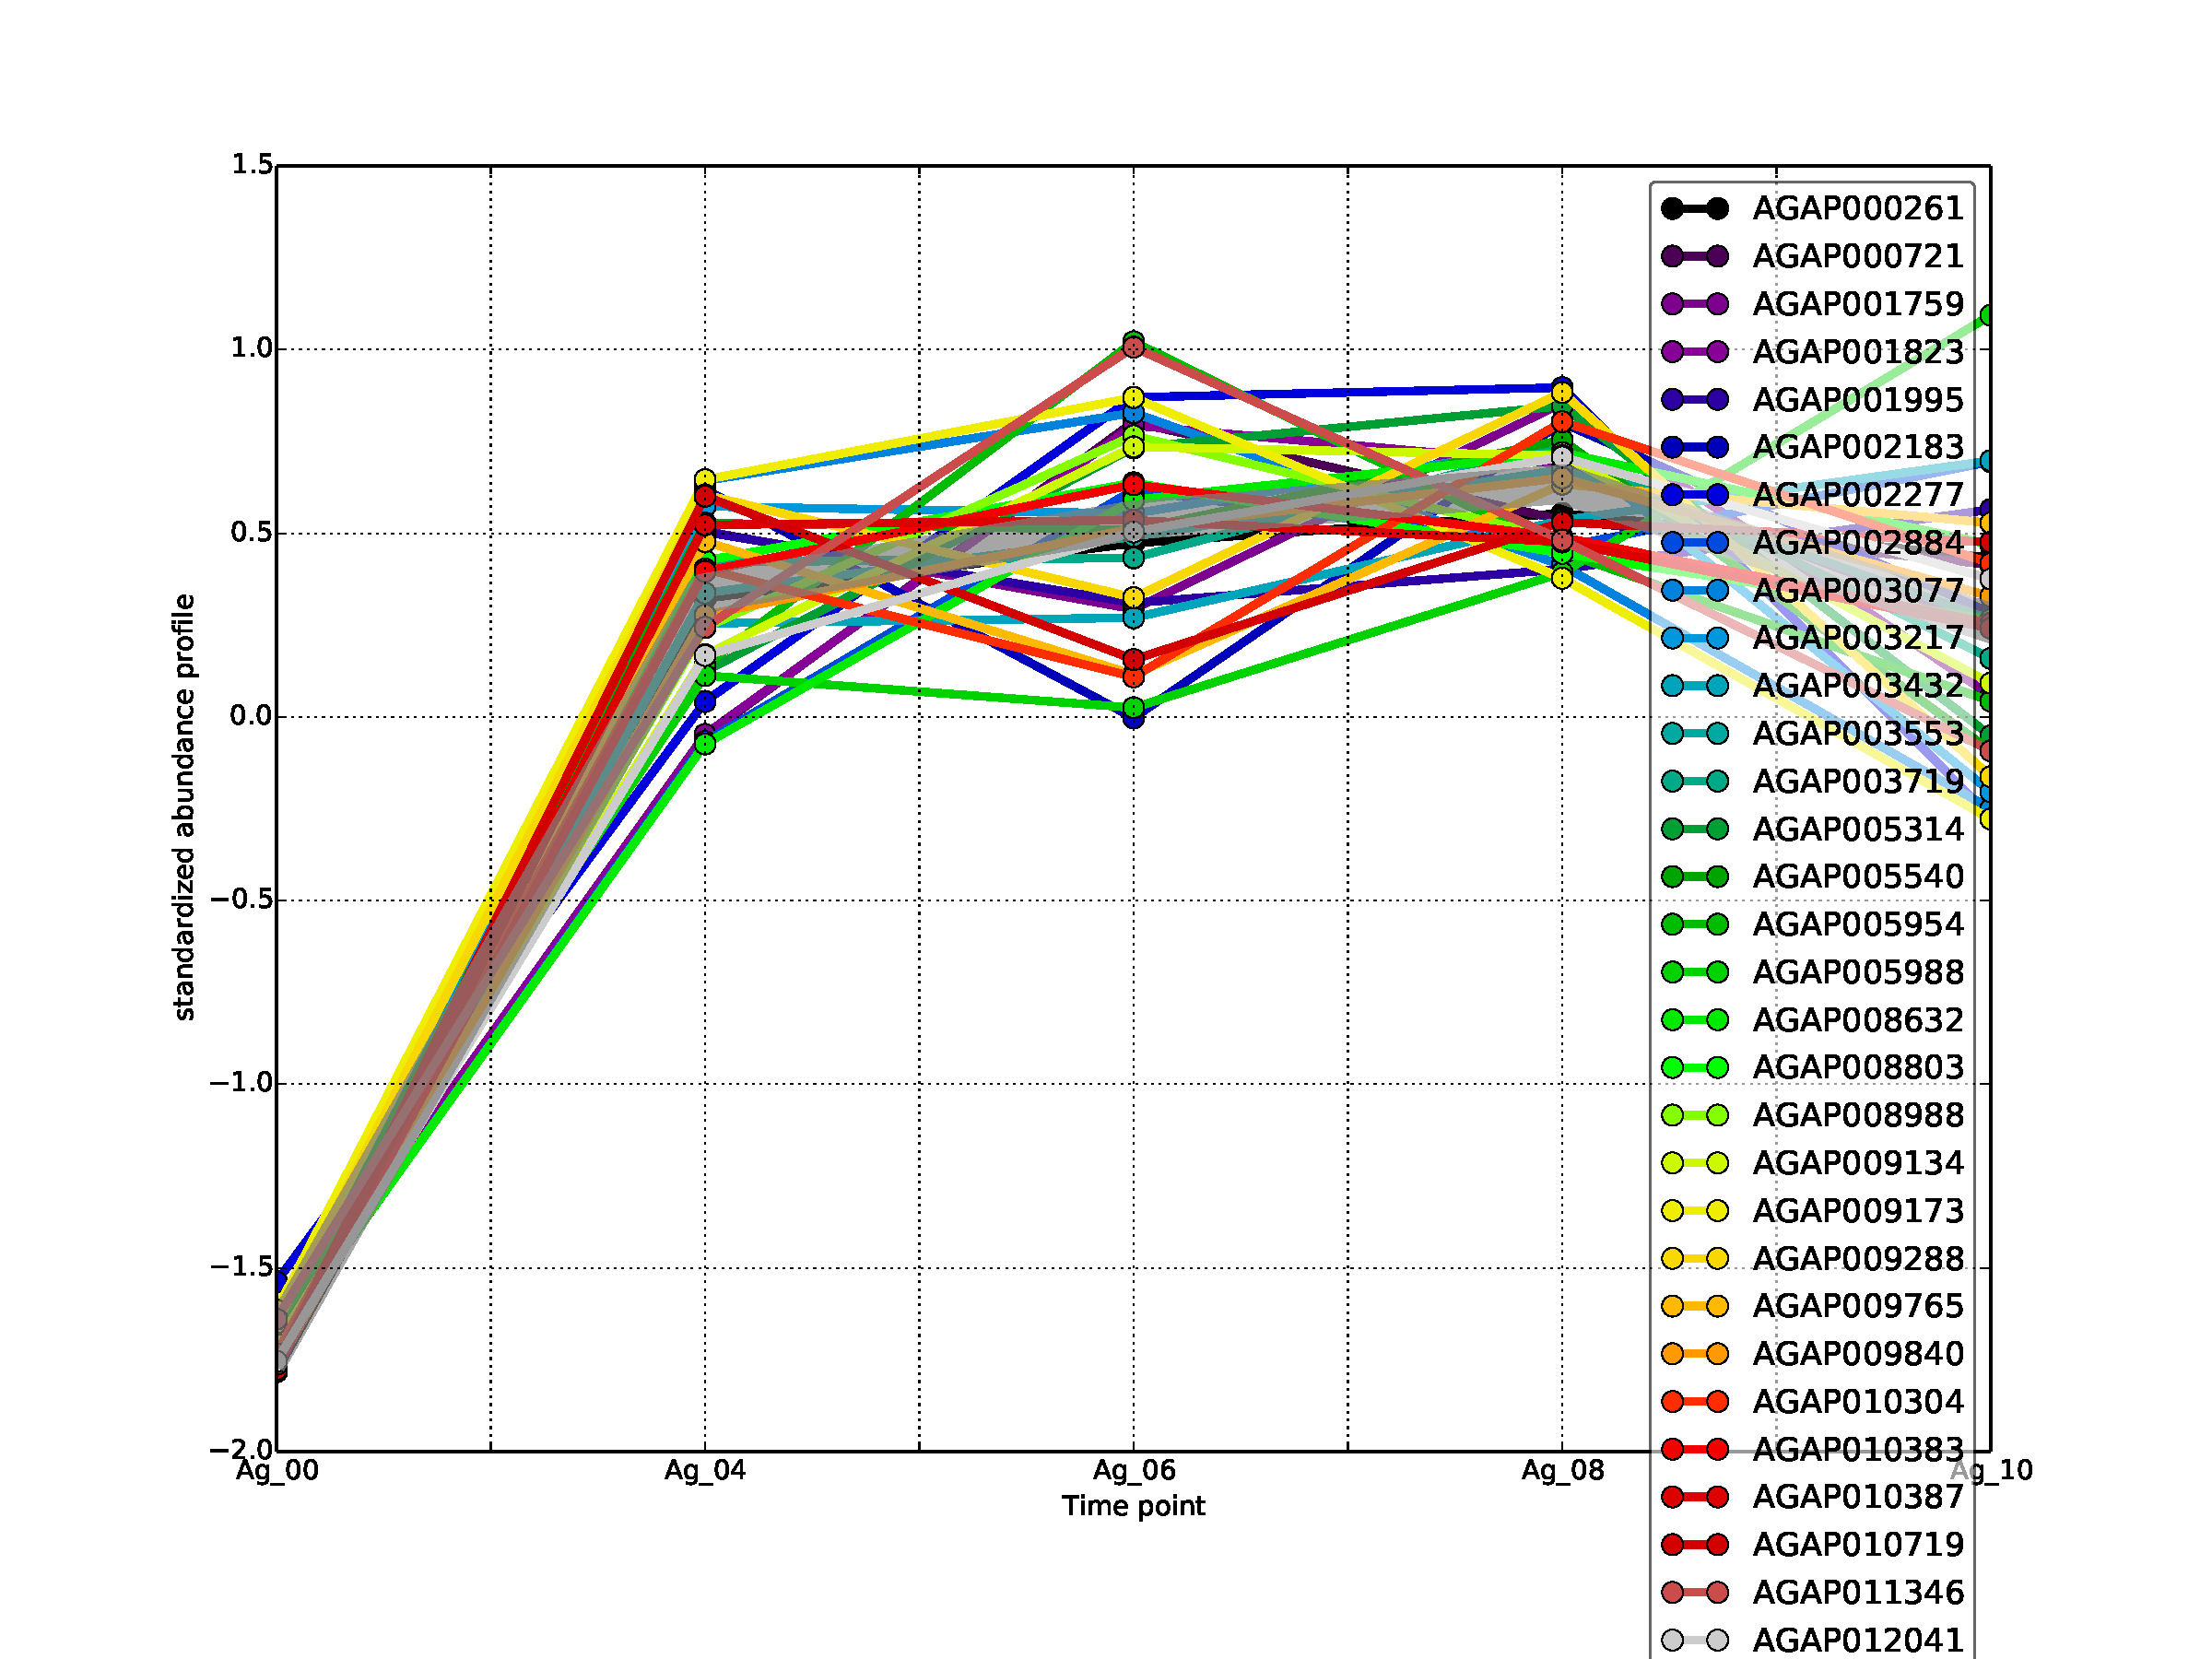
\includegraphics[width=\linewidth]{figures/figs/ecr_and_insects_ptci_20130903/upAfter4_gene_profiles_from_cummerbund/Ag_upAfter4_cls7_Ag_target_FPKMs_vb_orthos.pdf}
\caption{}
\label{fig:cluster7-Ag}
\end{subfigure}
% 
\begin{subfigure}[t]{.5\linewidth}
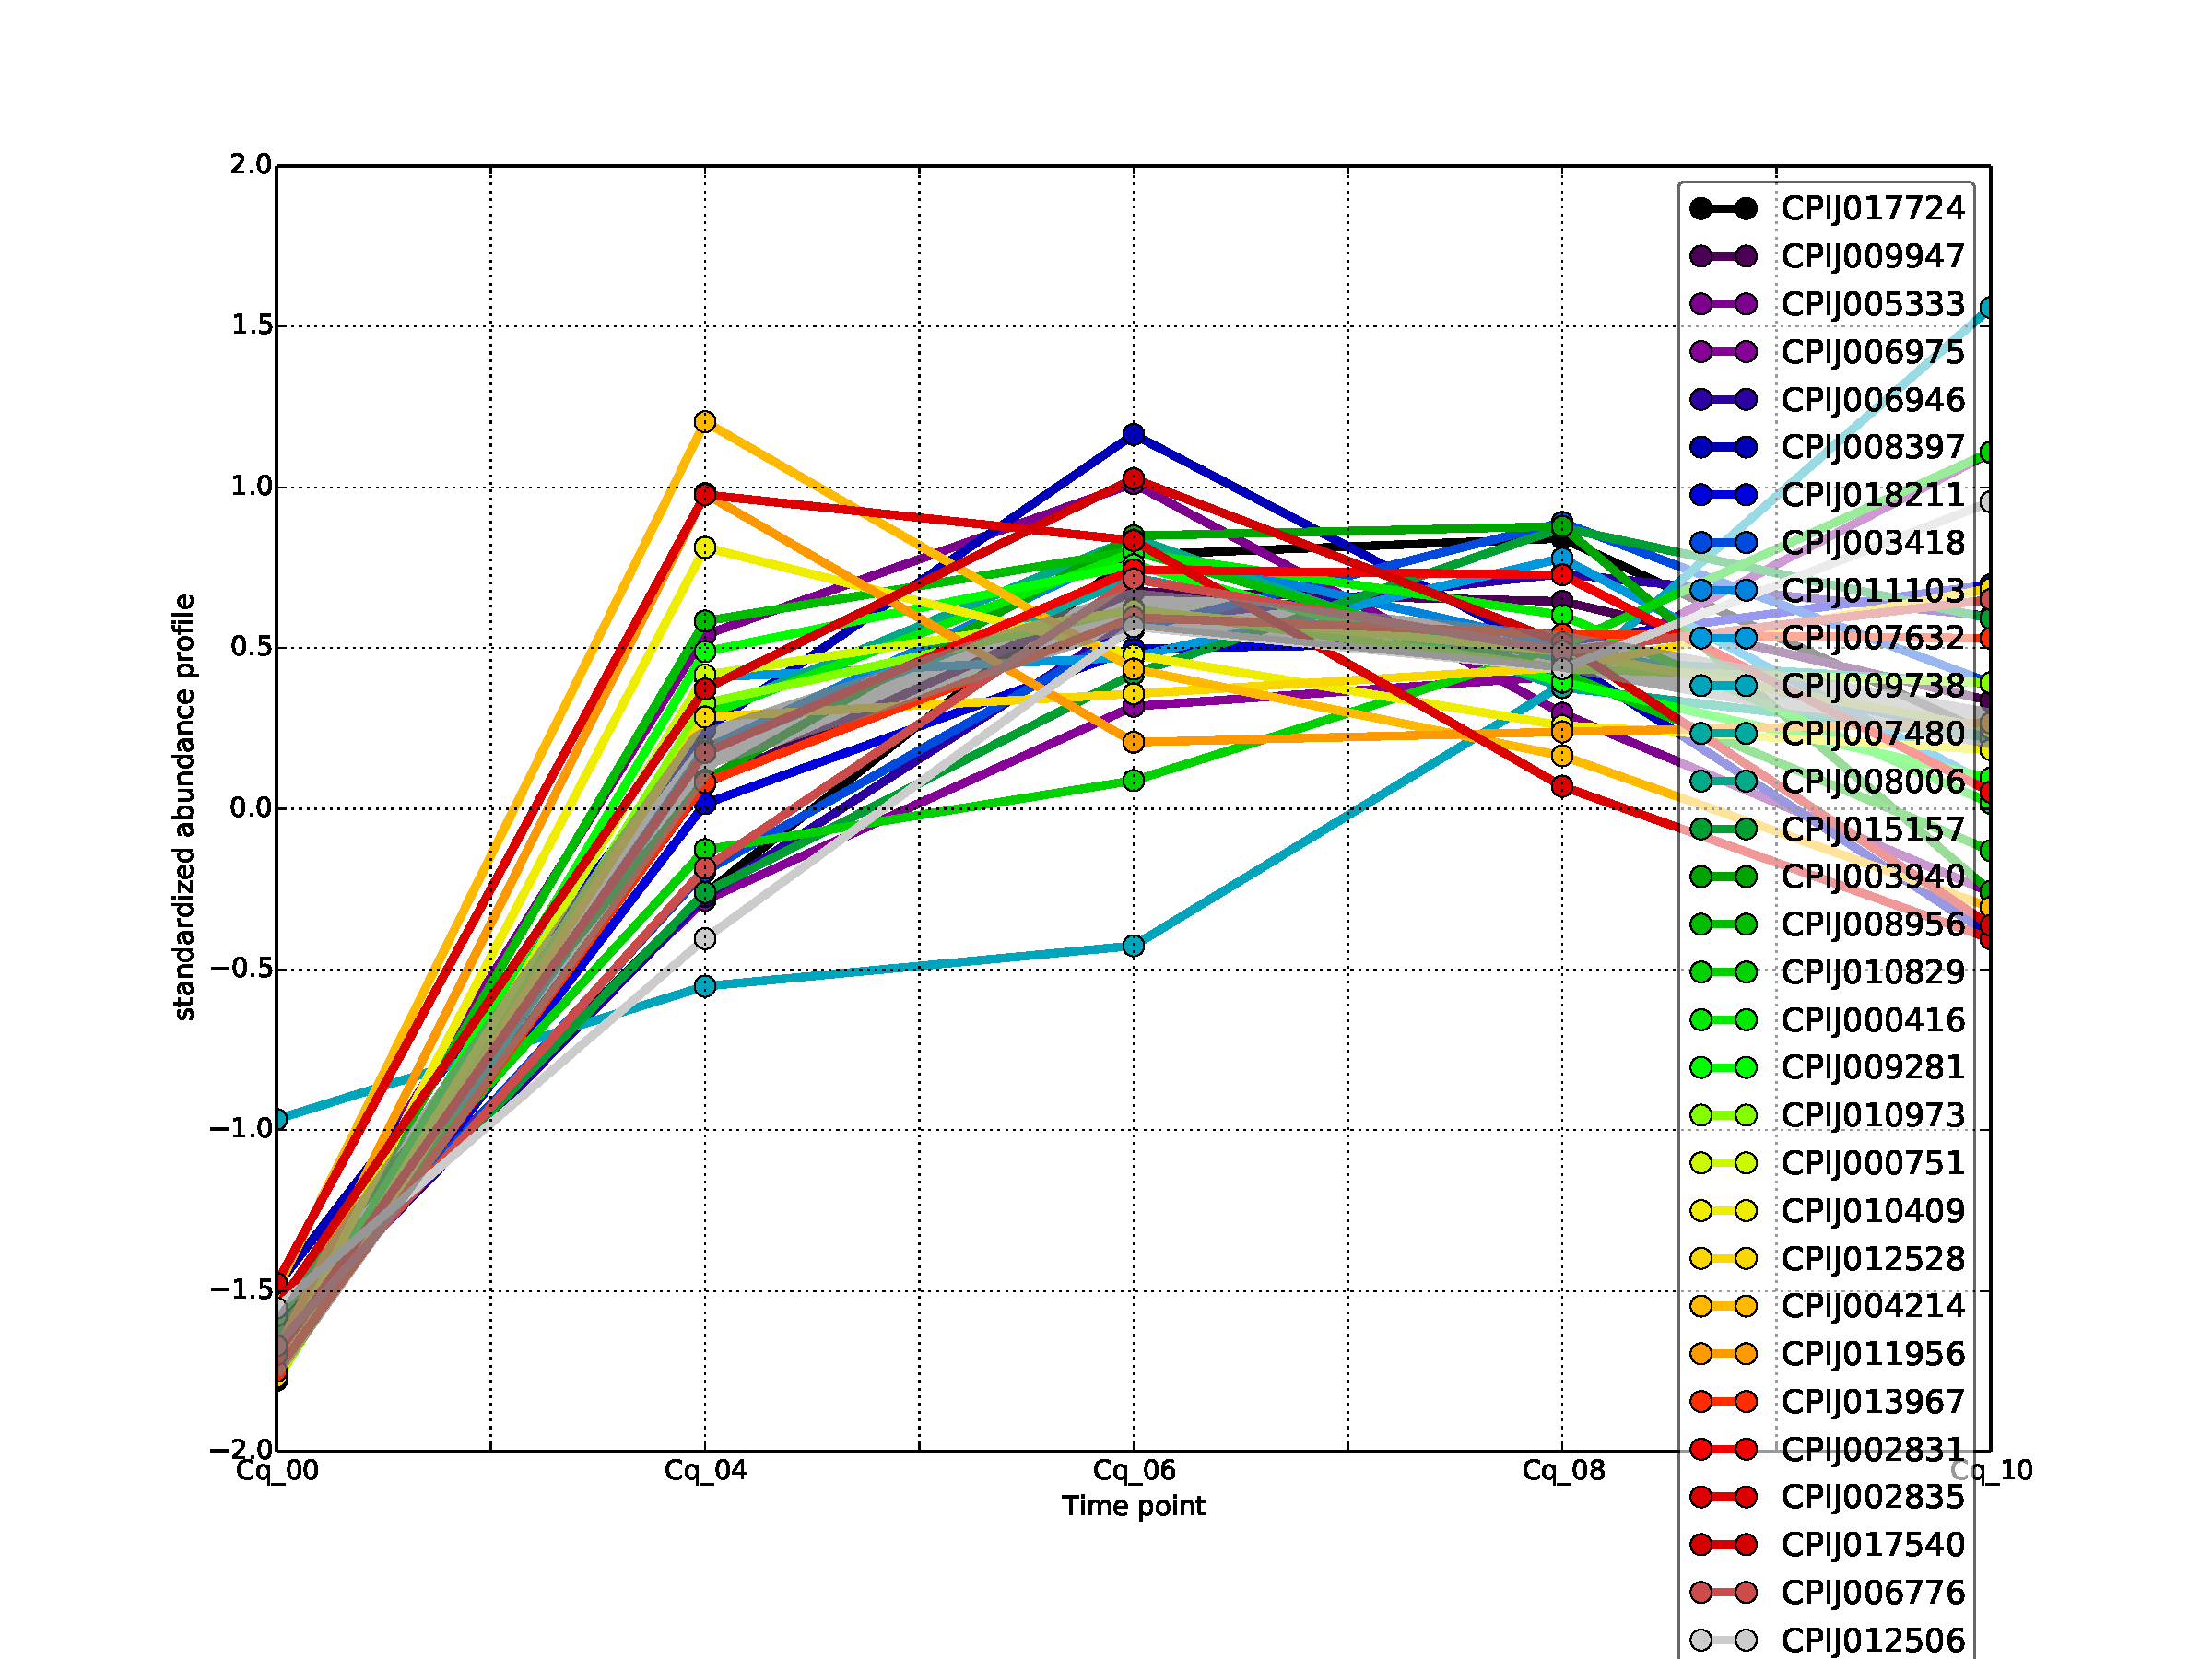
\includegraphics[width=\linewidth]{figures/figs/ecr_and_insects_ptci_20130903/upAfter4_gene_profiles_from_cummerbund/Cq_upAfter4_cls7_Ag_target_FPKMs_vb_orthos.pdf}
\caption{}
\label{fig:cluster7-Cq}
\end{subfigure}
% 
\caption[Orthologs of cluster 7]{\sf \textbf{Orthologs of cluster 7:}\\

\textbf{(A)} \Aa.
\textbf{(B)} \Ag.
\textbf{(C)} \Cq.
\todo[inline,caption={Finish Fig \ref{fig:cluster7}}]{ 
\begin{itemize}
    \item the text
    \item double gene names
    \item fix fig widths
\end{itemize}}
}
\label{fig:cluster7}
\end{figure}
% Figure \ref{fig:cluster7}
% 
% \input{/home/gus/Dropbox/common/projects/Aa_Ag_Cq_As/gfunc_stuff/prelim_gene_analysis/ecr_OR_insect_20130903/ptci_1_0/clusters/cls7/pandas_out/process.tex}
% Table \ref{tab:cluster7-P-mean-TS}
% 
% 
% 
\begin{figure}[hp]
% 
\begin{subfigure}[t]{.5\linewidth}
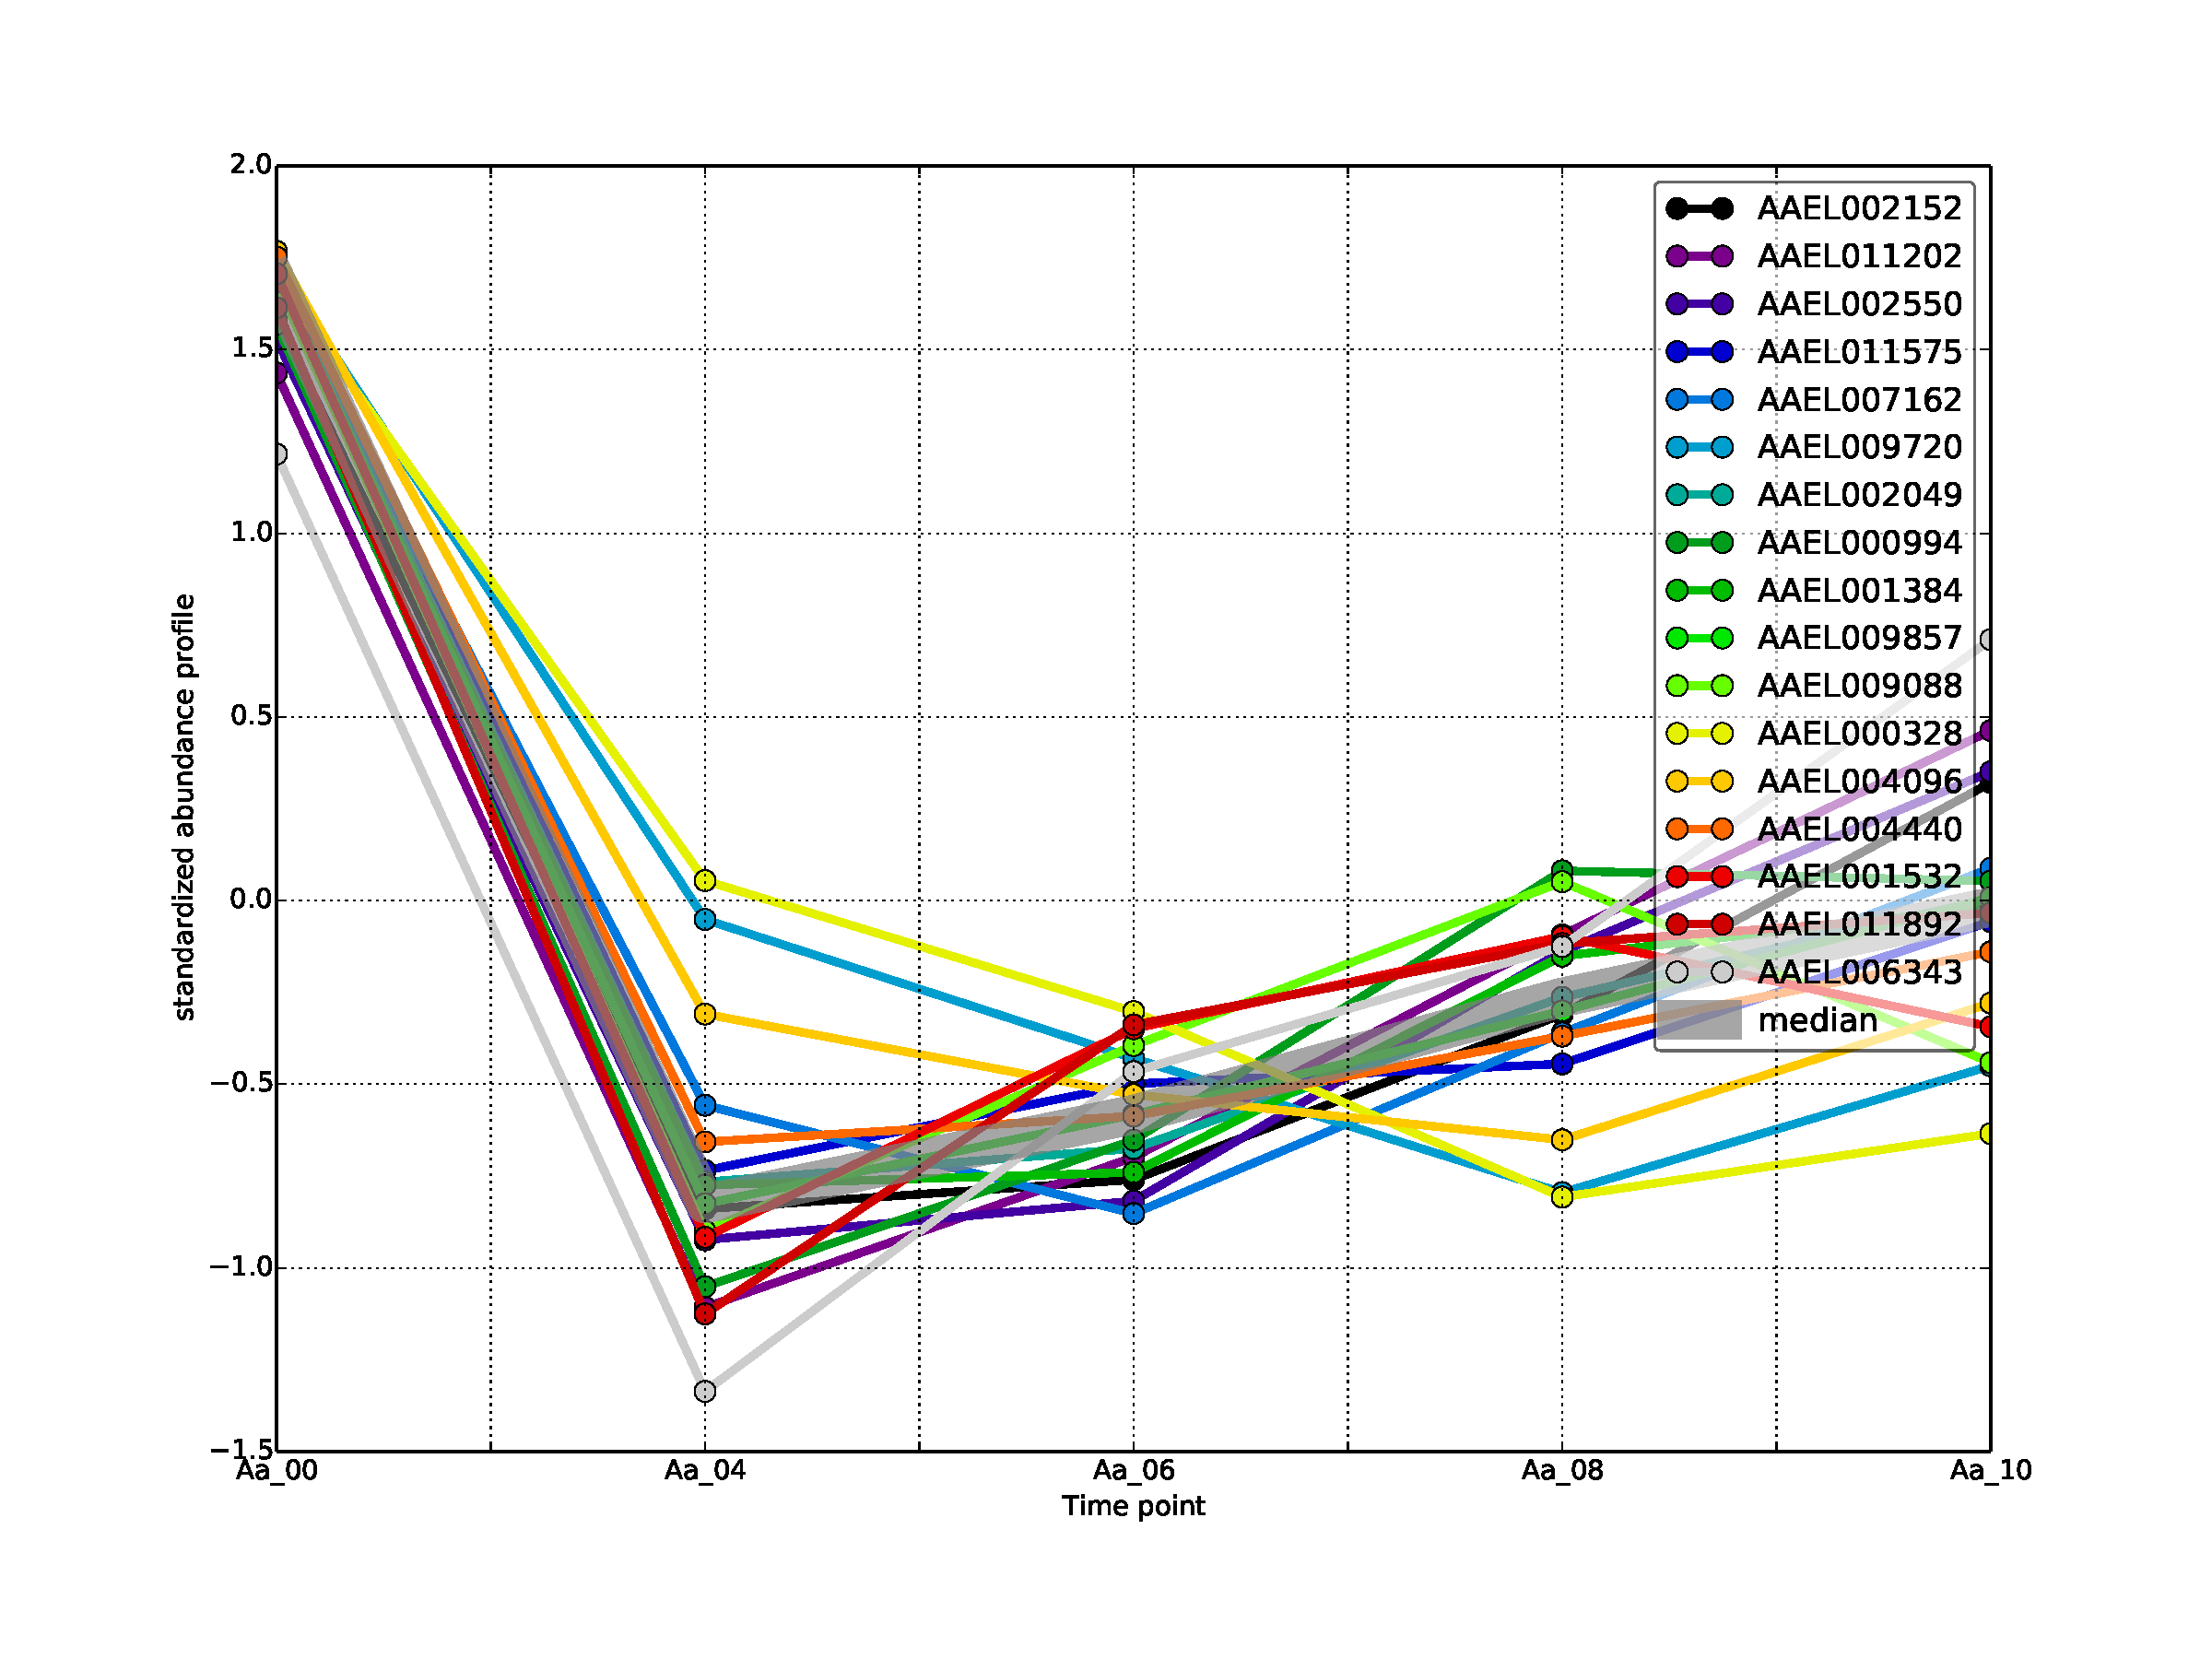
\includegraphics[width=\linewidth]{figures/figs/ecr_and_insects_ptci_20130903/downAt4_gene_profiles_from_cummerbund/Aa_downAt4_cls19_Ag_target_FPKMs_vb_orthos.pdf}
\caption{}
\label{fig:cluster19-Aa}
\end{subfigure}%
%
\begin{subfigure}[t]{.5\linewidth}
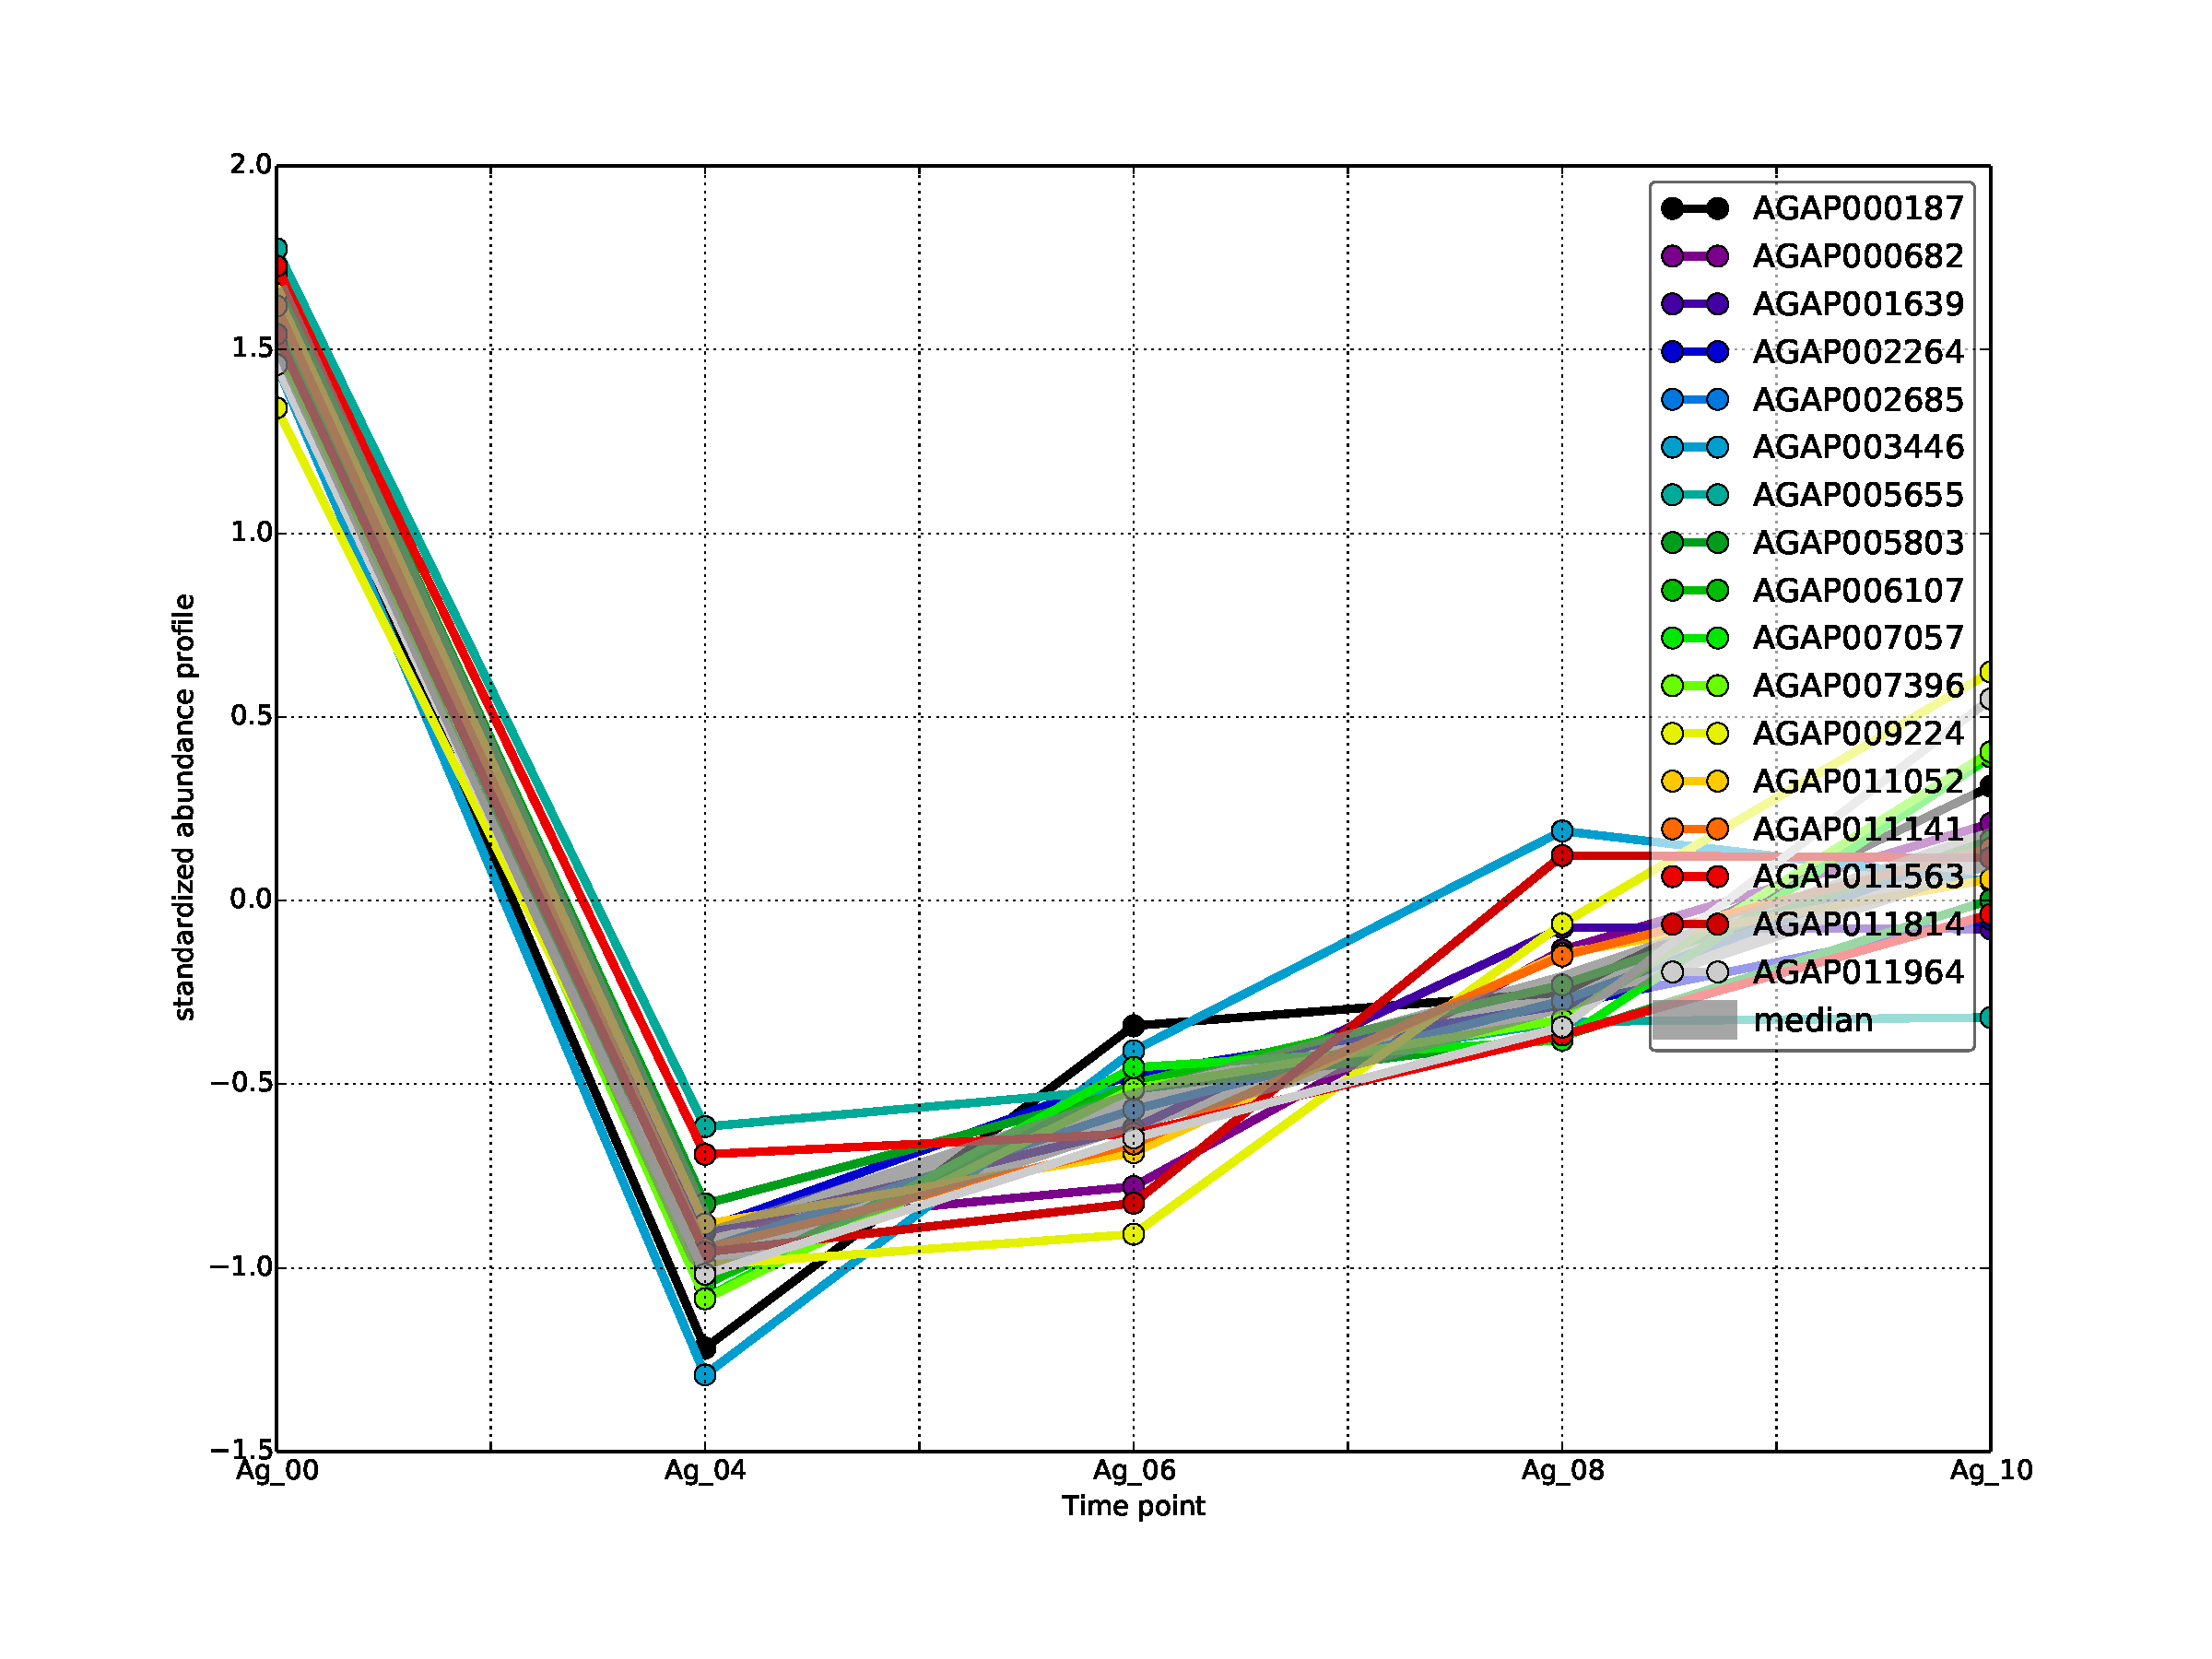
\includegraphics[width=\linewidth]{figures/figs/ecr_and_insects_ptci_20130903/downAt4_gene_profiles_from_cummerbund/Ag_downAt4_cls19_Ag_target_FPKMs_vb_orthos.pdf}
\caption{}
\label{fig:cluster19-Ag}
\end{subfigure}
% 
\begin{subfigure}[t]{.5\linewidth}
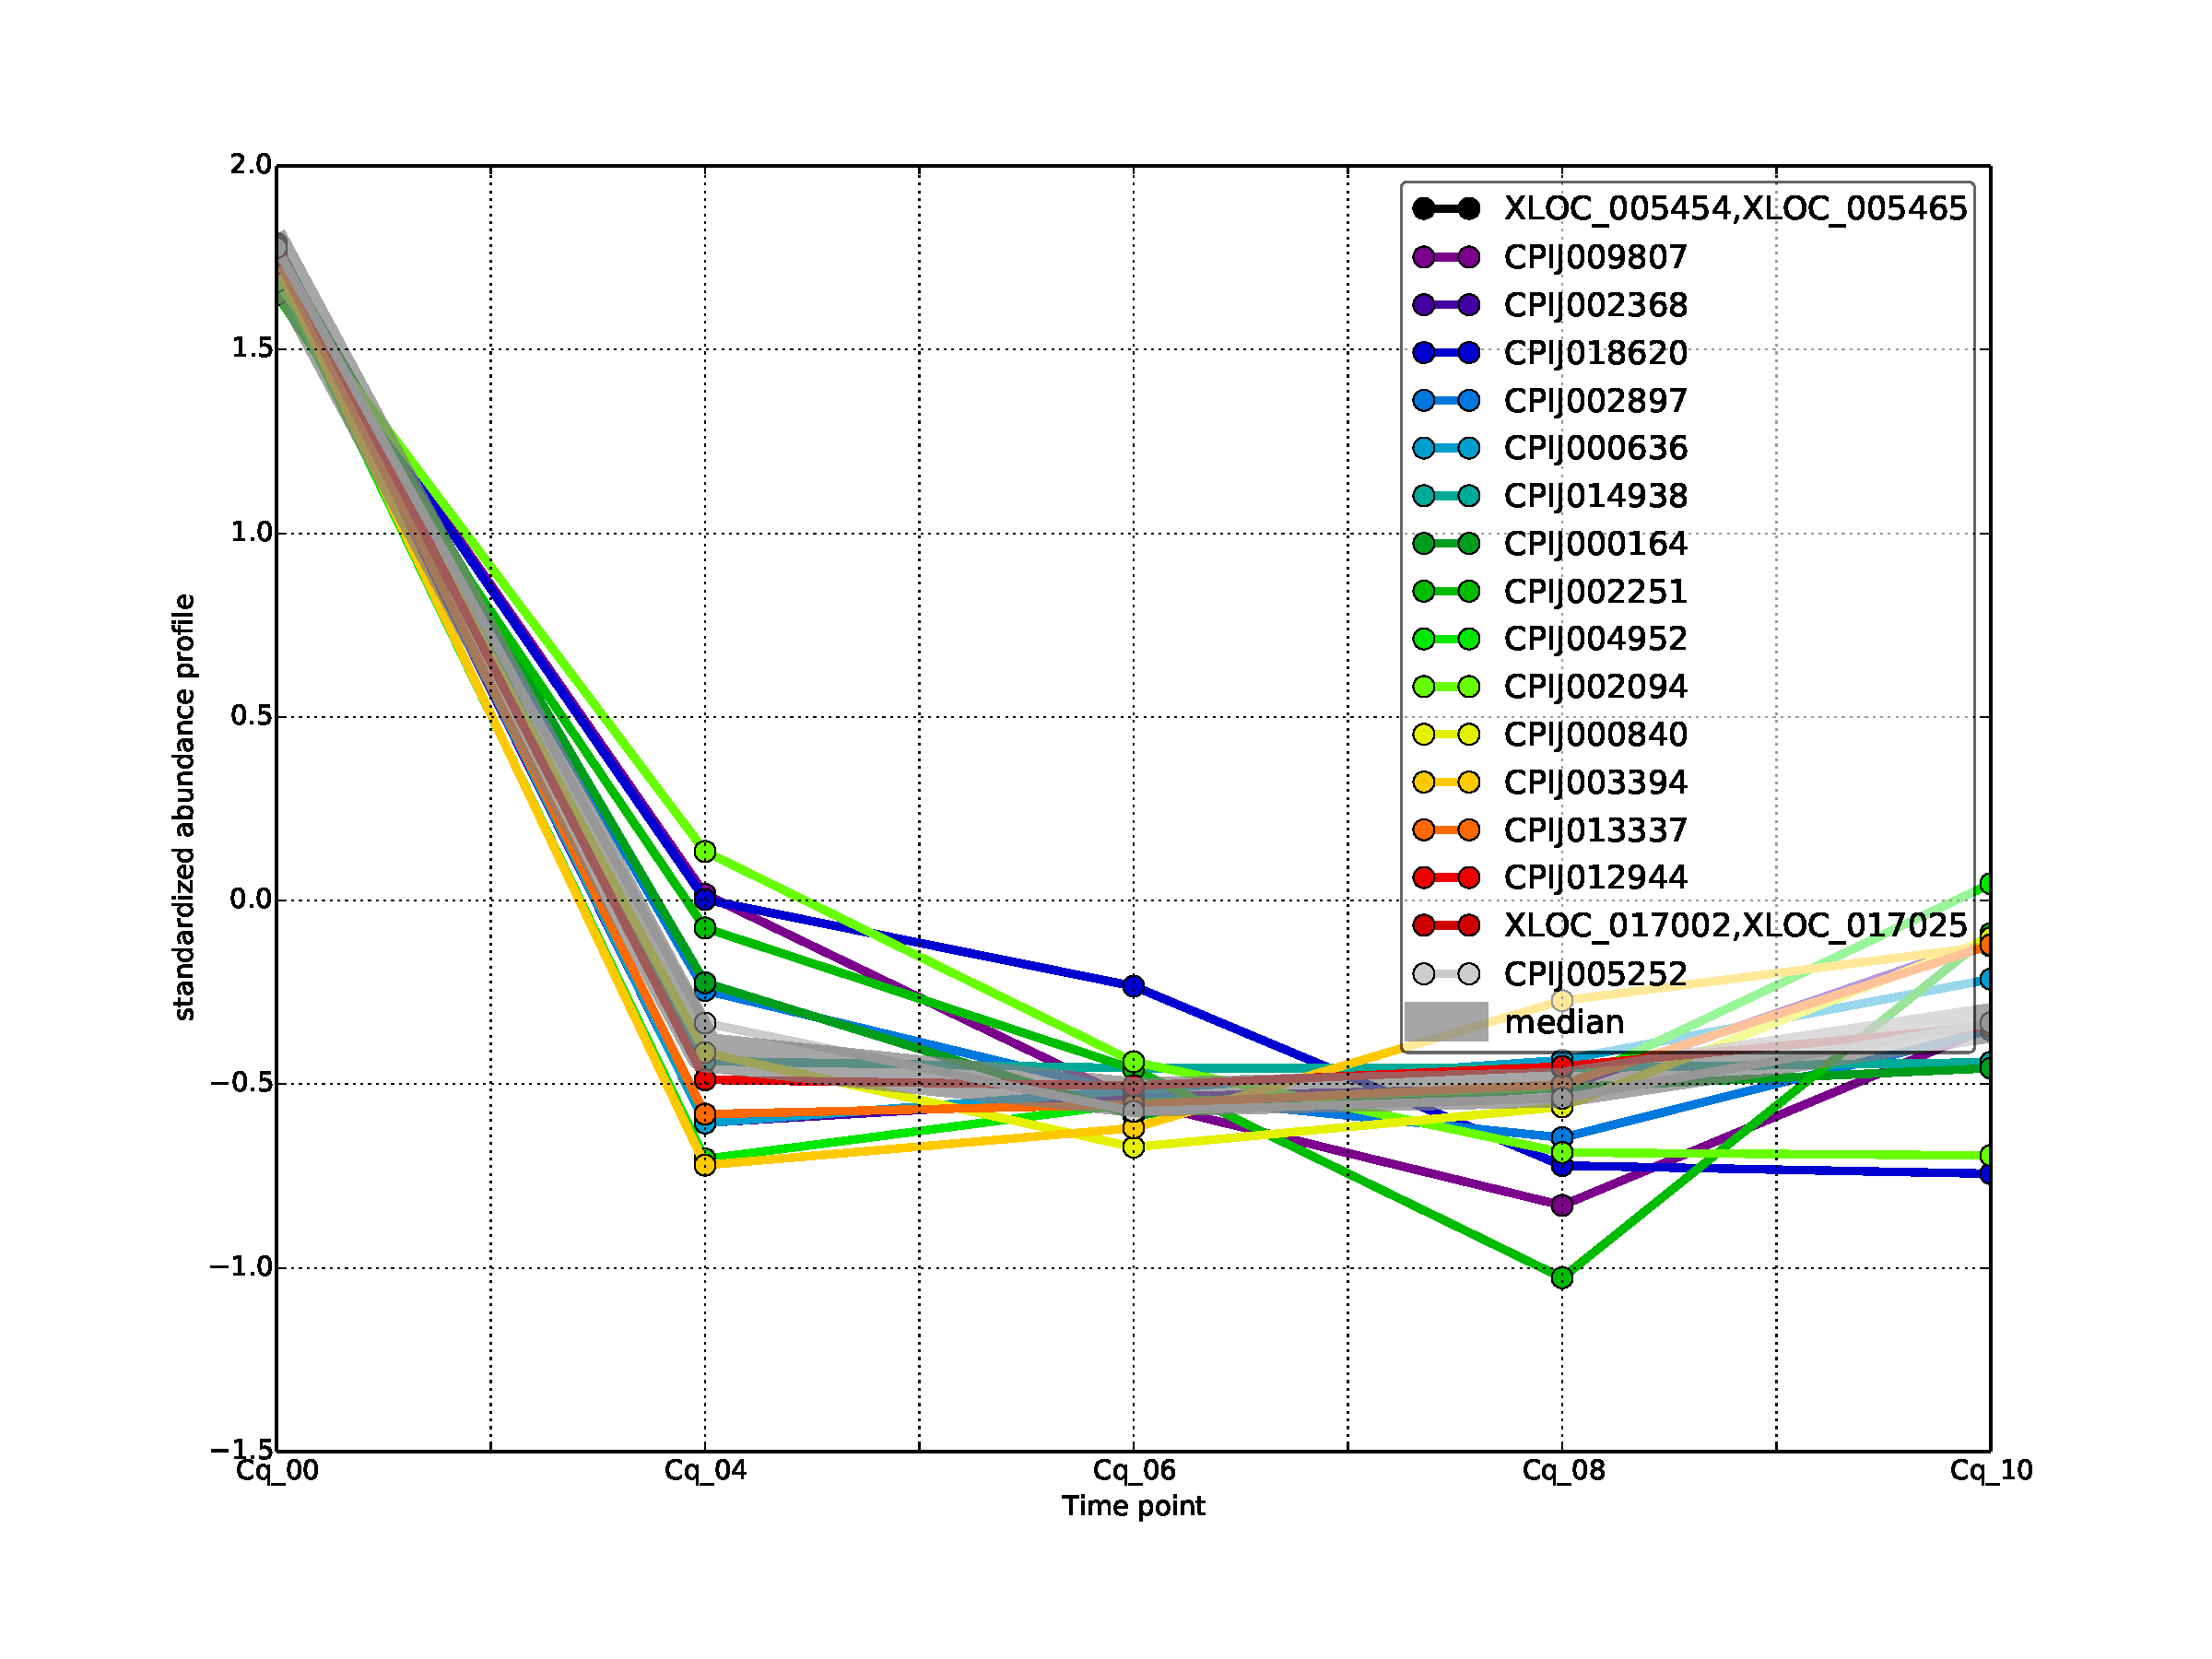
\includegraphics[width=\linewidth]{figures/figs/ecr_and_insects_ptci_20130903/downAt4_gene_profiles_from_cummerbund/Cq_downAt4_cls19_Ag_target_FPKMs_vb_orthos.pdf}
\caption{}
\label{fig:cluster19-Cq}
\end{subfigure}
% 
\caption[Orthologs of cluster 19]{\sf \textbf{Orthologs of cluster 19:}\\

\textbf{(A)} \Aa.
\textbf{(B)} \Ag.
\textbf{(C)} \Cq.
\todo[inline,caption={Finish Fig \ref{fig:cluster19}}]{Finish this fig: 
\begin{itemize}
    \item the text
    \item double gene names
    \item fix fig widths
\end{itemize}}
}
\label{fig:cluster19}
\end{figure}
% Figure \ref{fig:cluster19}



%%% Local Variables: ***
%%% mode: latex ***
%%% TeX-master: "thesis.tex" ***
%%% End: ***
